% !TeX spellcheck = en_US 
\chapter{Validation}\label{Validation}
This chapter covers the implementation and results of the proposed method in chapter \ref{MET}.

\section{Implementation}
\subsection{General Information regarding the Implementation}
The method is implemented in Python 3.9.9 for its widespread availability of libraries for ML-algorithms.
The libraries from which the classifier and regressors are taken are "scikit-learn" \cite{SKlearn}, "TSlearn" \cite{tslearn} and "xgboost" \cite{XG}.
Multiple models are tested and compared regarding their performance. %Runtime comparisons are not performed.
\subsection{Data Cleanup}
The first step is the cleanup of the data and its translation into a more flexible format. The recordings of the load sequences are provided in a text-file format that includes information such as displacements of the piston, cycle-time and cycle-count.
Figure \ref{fig:recordinglabel} shows all the labels of the recorded values in the txt-file and their interpretation. All information is disregarded except the net force at each cycle-peak. The net force is the clamping force (lowest acting force) plus the recorded absolute peak (highest acting force). The order of loads is kept and the absolute values are transformed into an array that is stored as a NumPy file. 14 load sequences are available, which are transformed into 14 np-files and stored in a new folder. The np-file format allows for faster read times and takes up less space on the hard drive than the original txt-files. The names are not important and are thus also replaced by a simple index.


\begin{figure}[H]
	\centering
	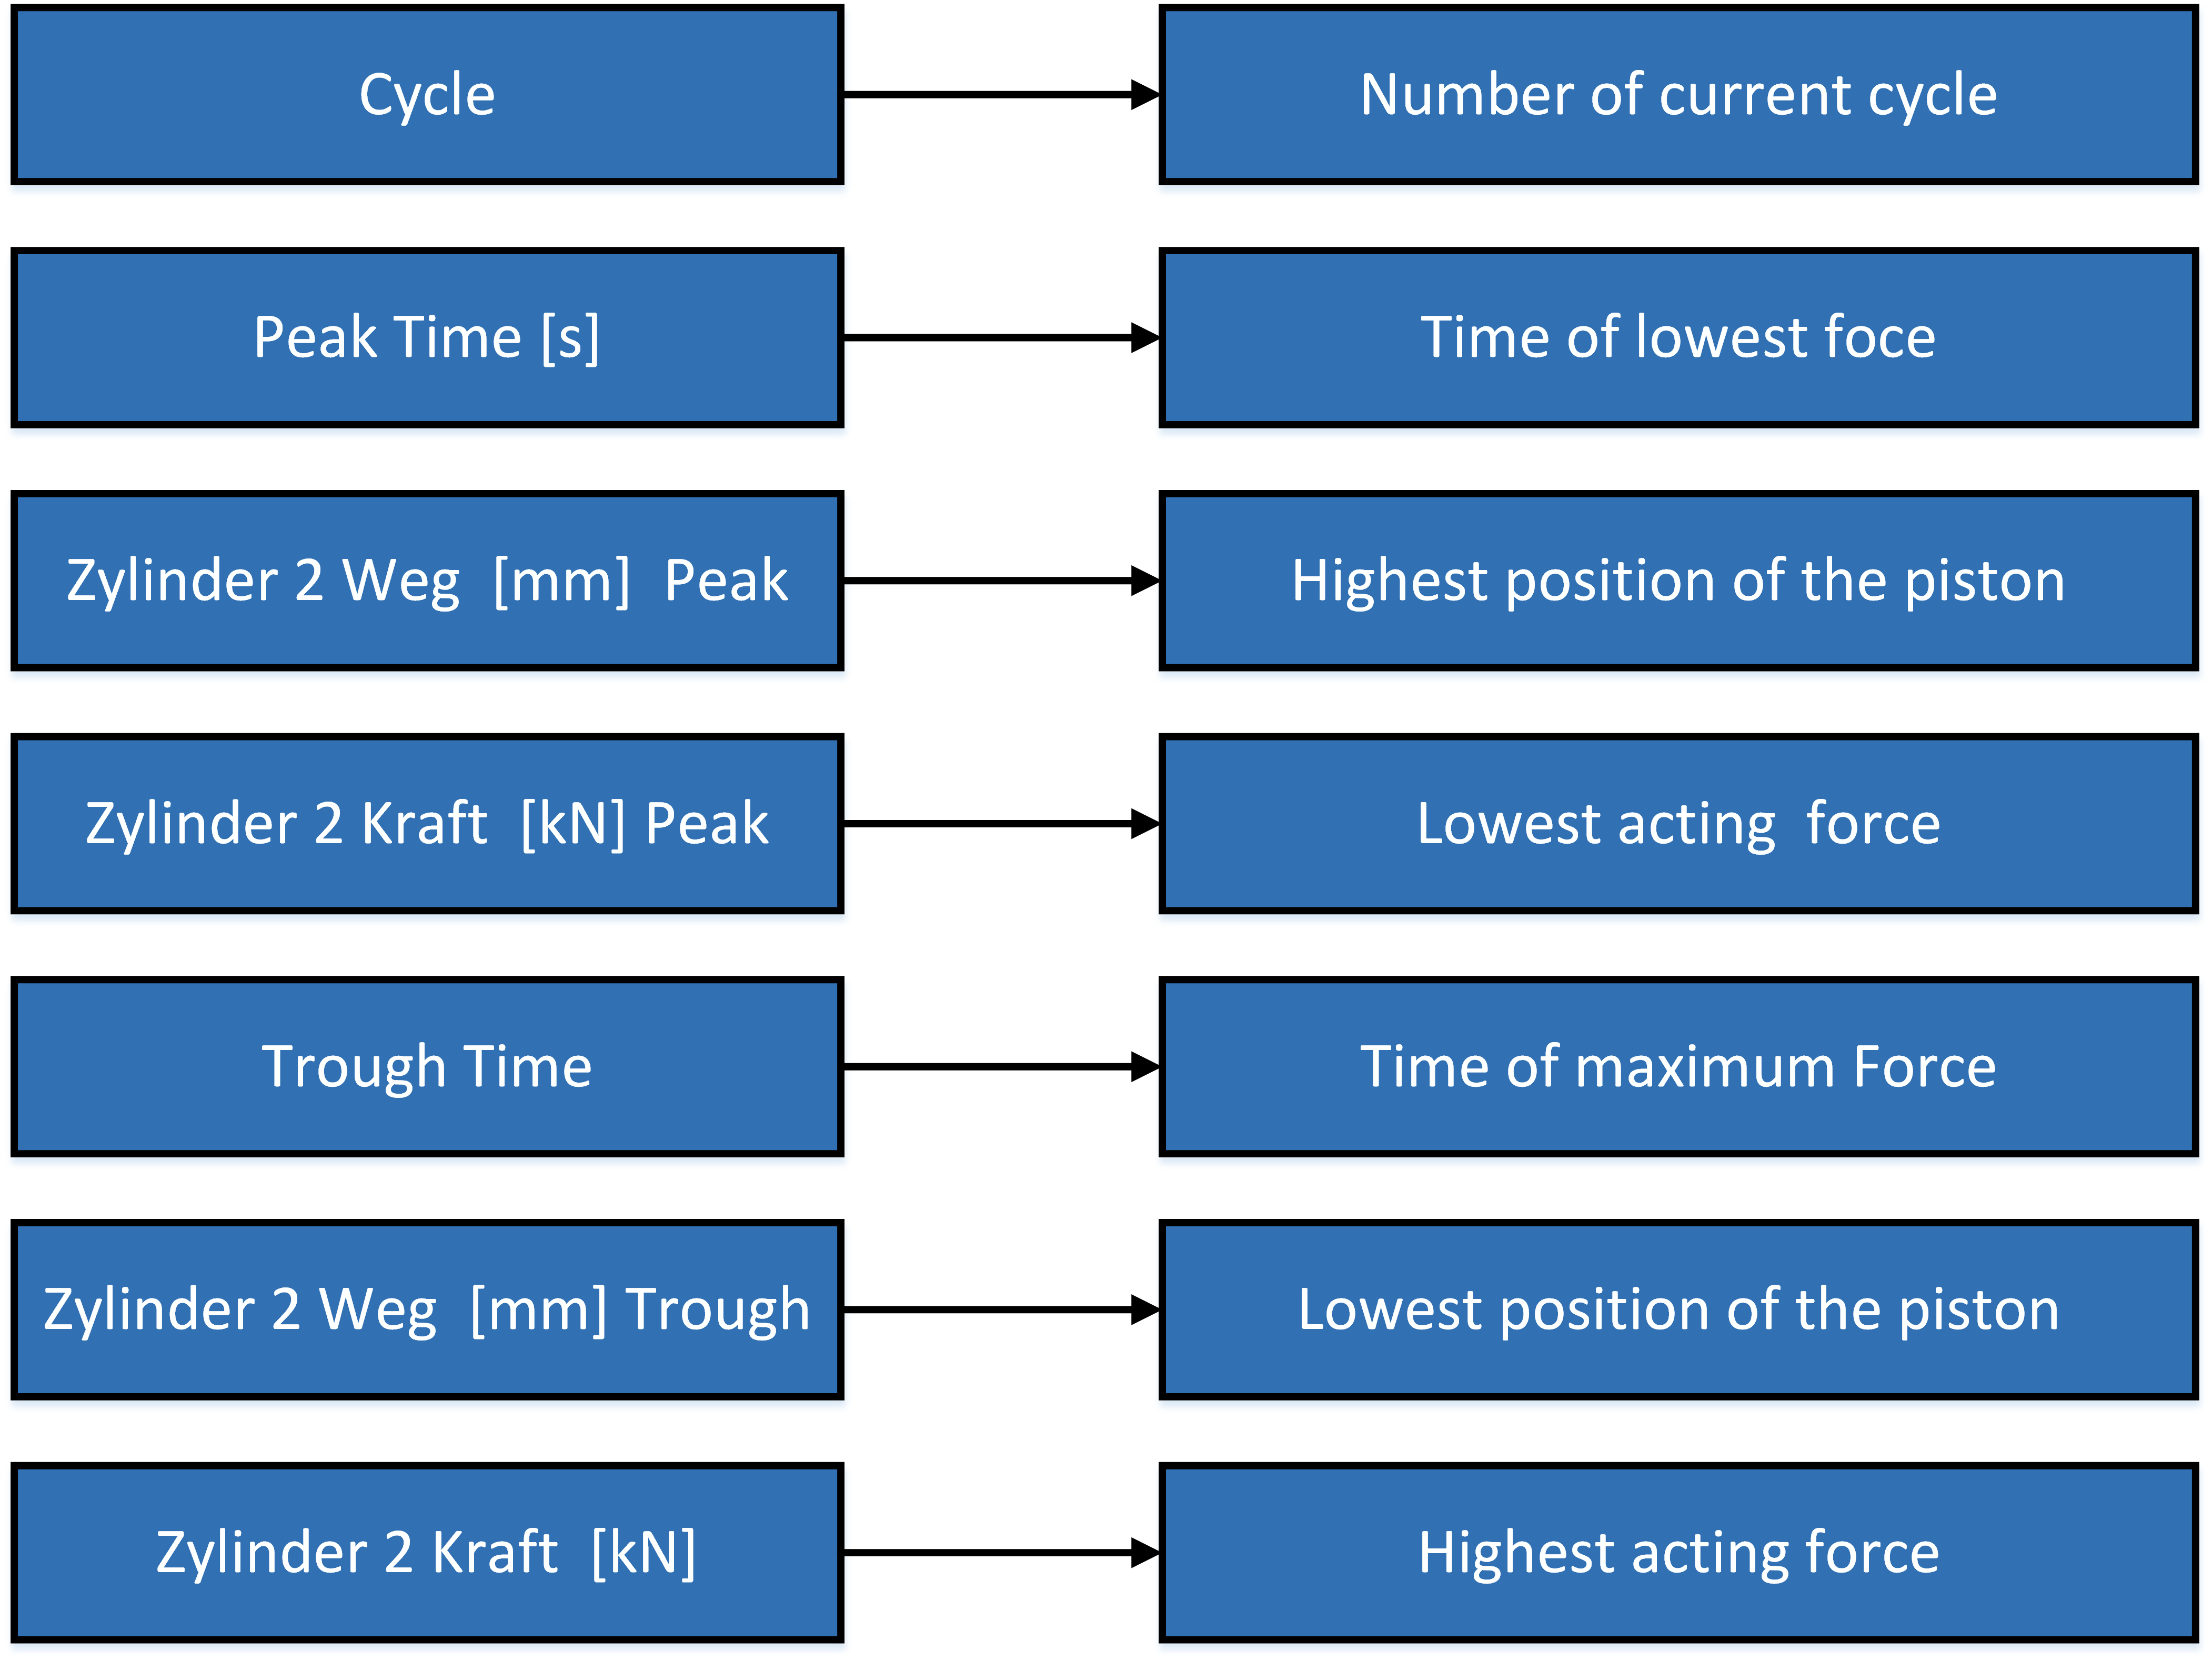
\includegraphics[width=0.75\linewidth]{IMGs/recordinglabel.png}
	\caption{Recorded parameters in STBF}
	\label{fig:recordinglabel}
\end{figure}

\subsection{Data Augmentation}
The data augmentation process starts with calculating the damage sum D with the help of the Basquin equation (see equation \ref{BQ}) and the Miner rule (see equation \ref{acc}).
The parameters for the Basquin equation were provided and shown in table \ref{paramBQ}.
Only forces higher than the endurance limit are selected when calculating the accumulated damage.  

The calculated damage sum D according to the Miner rule of the available files are shown in table \ref{DamageSUMS}


\begin{table}
	\begin{center}
		\begin{tabular}{|| r | l ||}
			\hline
			\rule{0pt}{2ex}Load Sequence Nr. & Damage sum D\\
			\hline
			\hline
			\rule{0pt}{2ex}0 & 2.16\\ \hline
			1 & 1.18\\	\hline
			2 & 1.29 \\ \hline
			3 & 0.92\\ \hline
			4 & 3.4 \\ \hline
			5 & 1.18 \\ \hline
			6 & 1.4 \\ \hline
			7 & 1.01 \\ \hline
			8 & 1.06 \\ \hline
			9 & 0.75 \\ \hline
			10 & 0.68 \\ \hline
			11 & 1.22\\ \hline
			12 & 0.73 \\ \hline
			13 & 1.1 \\ \hline
			\hline
		\end{tabular}
		\caption{Damage sum D at failure of available load sequences}
		\label{DamageSUMS}
	\end{center}
	\vspace{-4mm}
\end{table}


\begin{table}
	\begin{center}
		\begin{tabular}{|| l | l ||}
			\hline
			\rule{0pt}{2ex}Parameter D & Value\\
			\hline
			\hline
			\rule{0pt}{2ex}Slope of the S-N fatigue strength curve = k & 6.33048\\ \hline
			Reference value of fatigue strength = C & 11670367740000000\\	\hline
			Value of the load at one cycle = L & values from array \\ \hline
			Endurance limit & 56.618 kN \\ \hline
			\hline
		\end{tabular}
		\caption{Parameters of the Basquin-equation and Endurance Limit}
		\label{paramBQ}
	\end{center}
	\vspace{-4mm}
\end{table}

The first step in DA is the addition of random noise. A np-file is loaded and the damage~sum~D is calculated. That value serves as a reference to compare if the augmentation significantly changes the damage sum D.
The random noise is in the form of a vector that has the same length as the loaded load sequence.
The individual noise values follow a Gaussian distribution with a mean of 0 and a standard deviation of 0.2. 
The values of that noise vector are also in kN and thus can be simply added.
Figure \ref{fig:V5} shows a load sequence in its unedited form without the addition of noise. Figure \ref{fig:V5_noise} shows the same load sequence with the additional noise vector. As can be seen, the damage sum D is not changed enough to be noticeable when rounding to two decimal places. 

\begin{figure}[H]
	\centering
	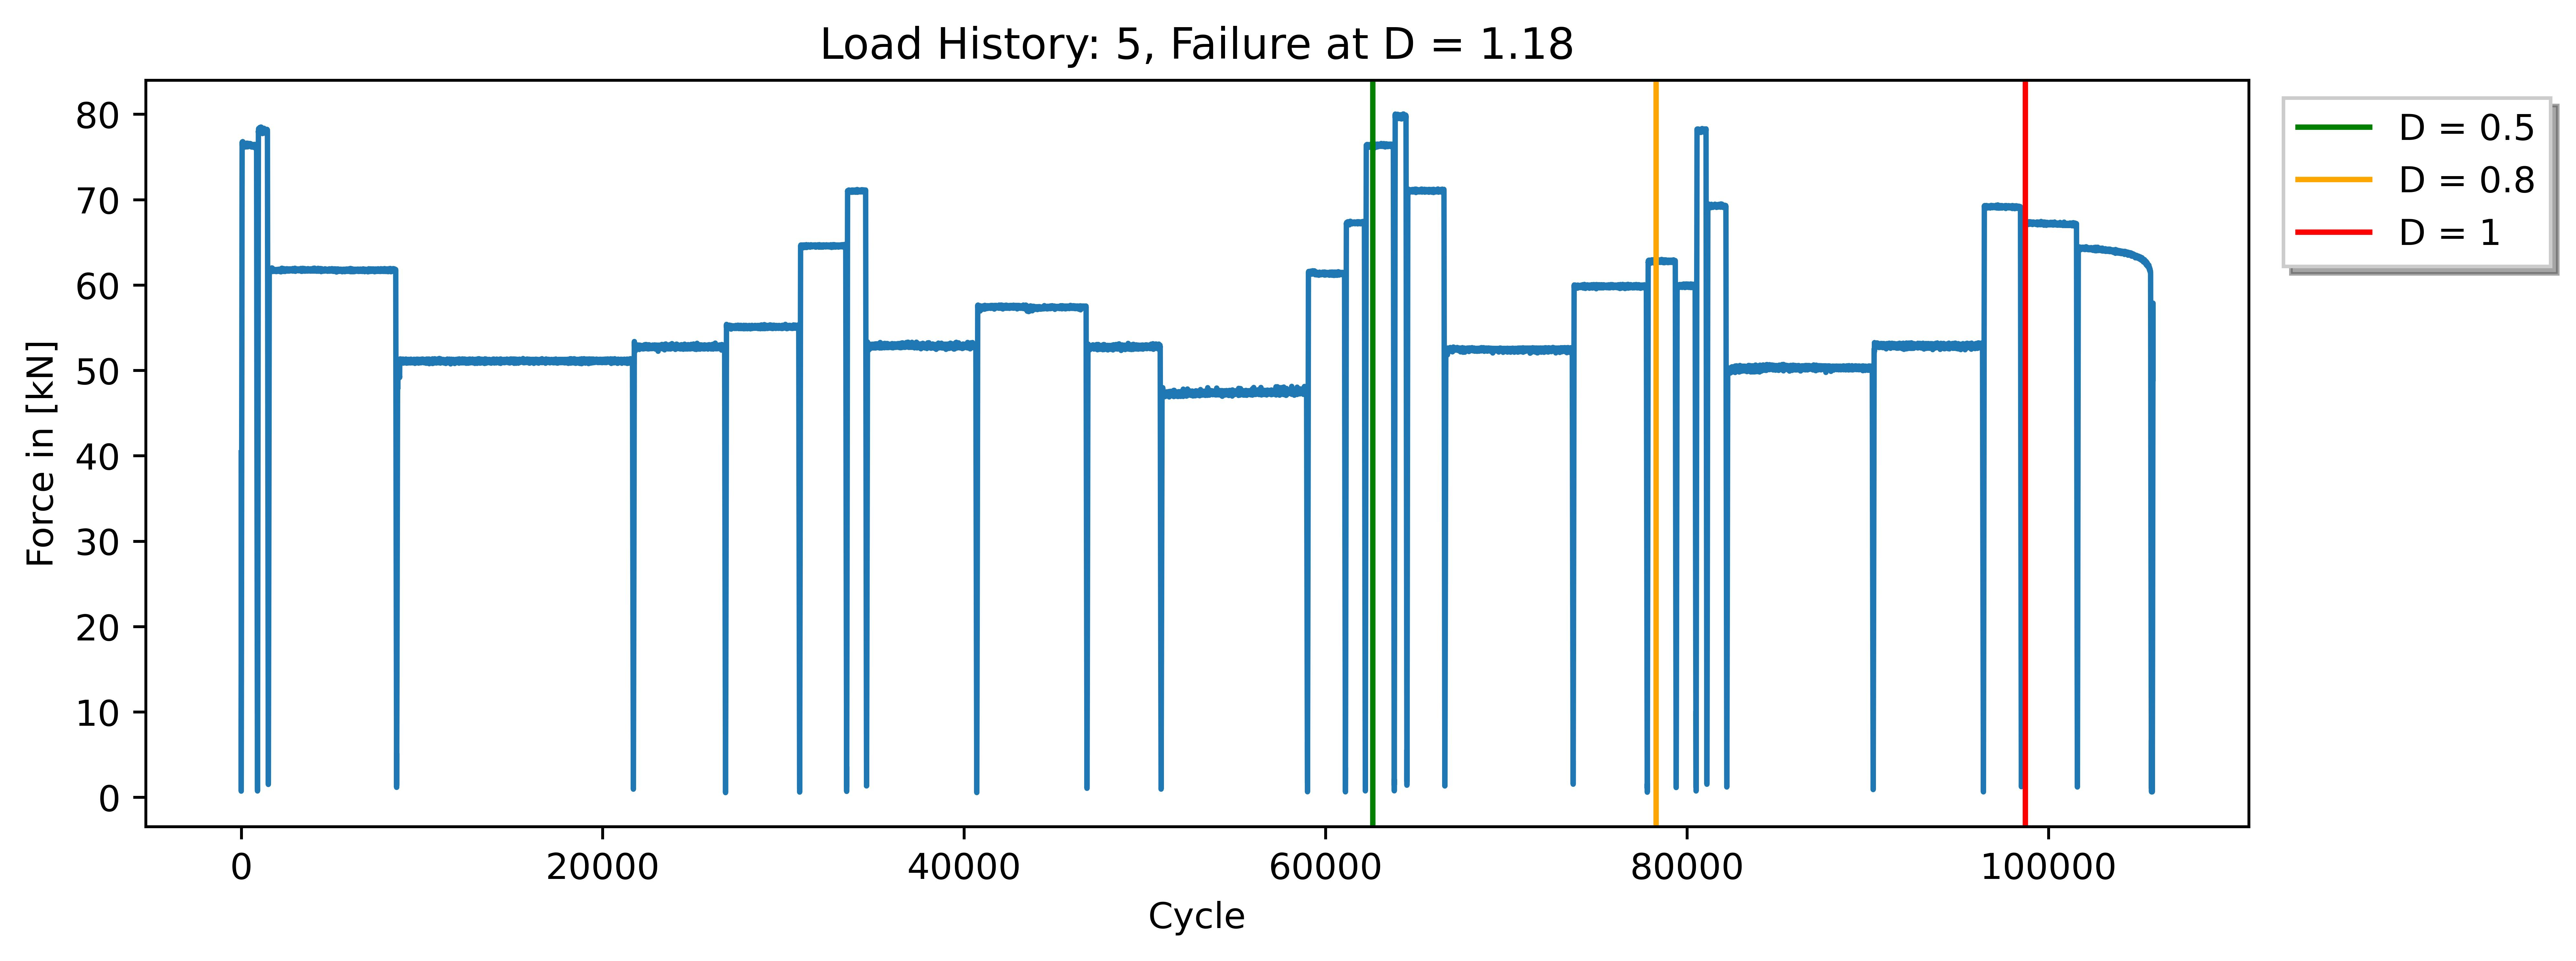
\includegraphics[width=1\linewidth]{IMGs/Verlauf_5.jpg}
	\caption{Load sequence without DA}
	\label{fig:V5}
\end{figure}

\begin{figure}[H]
	\centering
	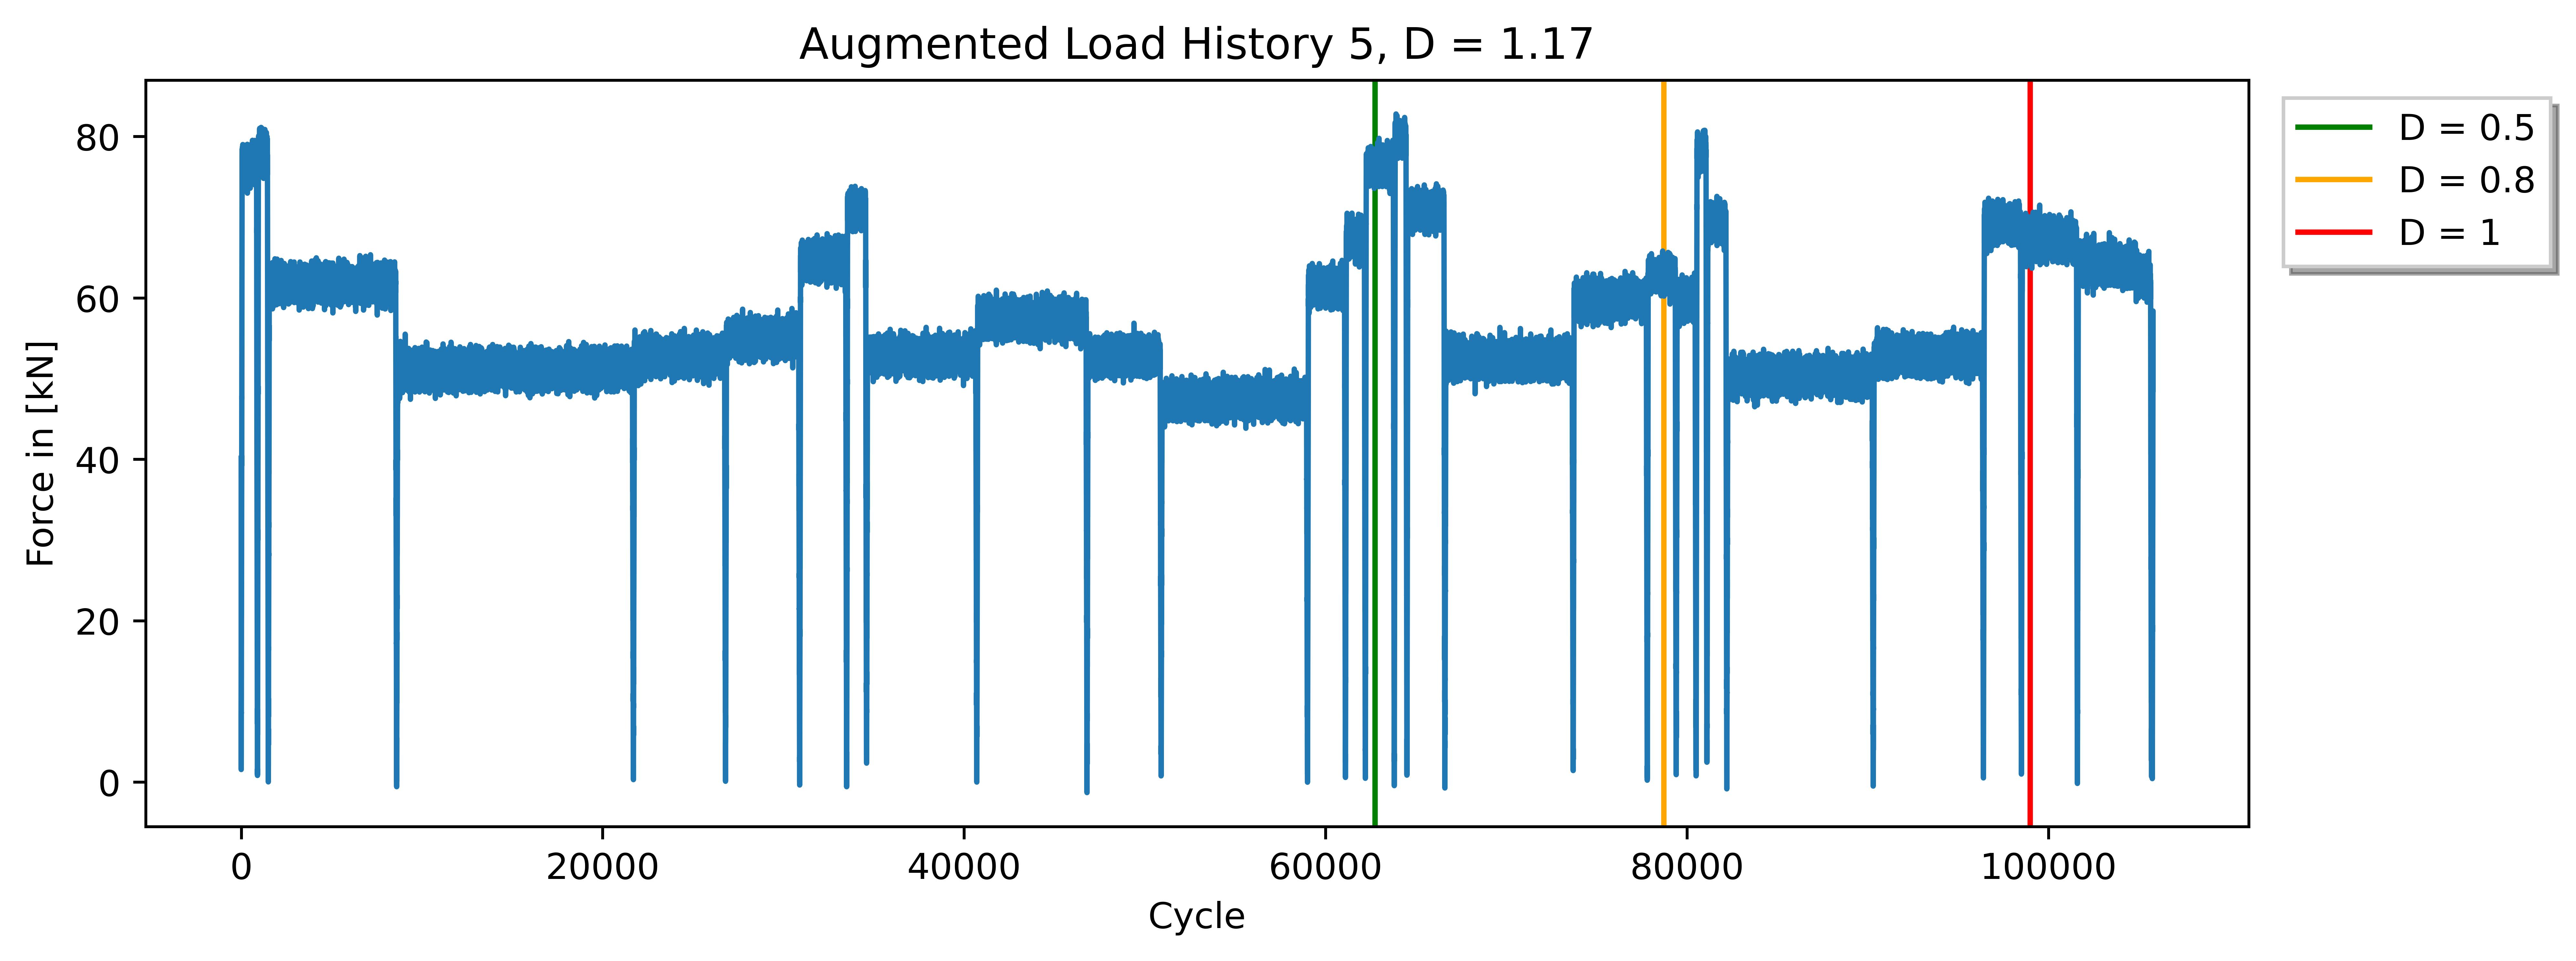
\includegraphics[width=1\linewidth]{IMGs/Verlauf_5_noise.jpg}
	\caption{Load sequence with additional noise}
	\label{fig:V5_noise}
\end{figure}

The second performed step is a global shift of the whole loading sequence up or down by up to 500 N. This is done by sampling a uniform distribution between -1 and 1 and multiplying by 0.5. This constant is added to every array element. Figure \ref{fig:V5_shift} shows the shifted load sequence with the previously added noise. In this case, the damage sum D is altered either in the negative or positive direction. Again, no significant changes occurred regarding damage sum D.

\begin{figure}[H]
	\centering
	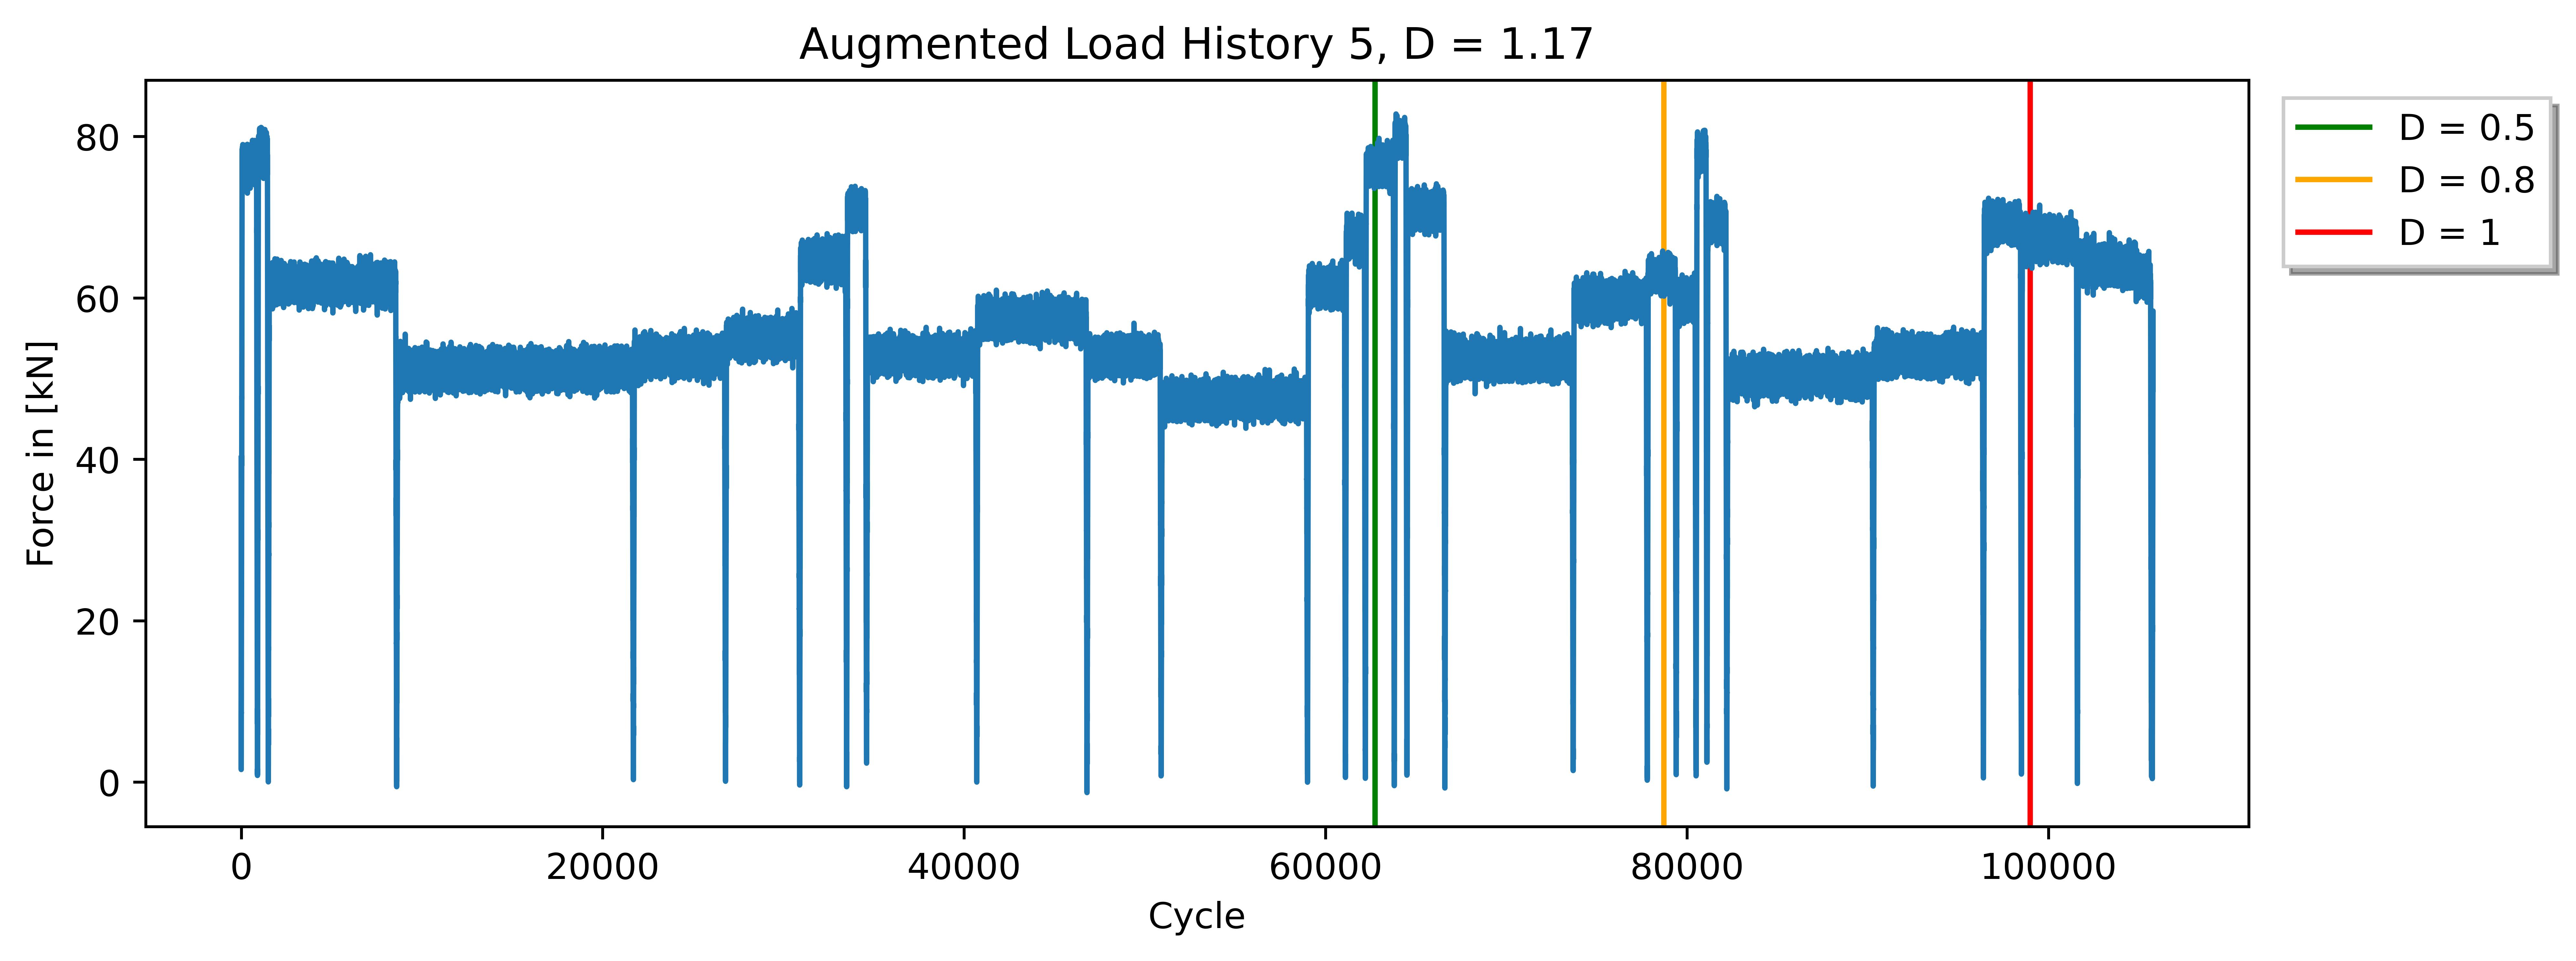
\includegraphics[width=1\linewidth]{IMGs/Verlauf_5_noise.jpg}
	\caption{Load sequence with noise and shift}
	\label{fig:V5_shift}
\end{figure}

The third step is a section-wise random shift. A random section of the array with a length of 1 \% of the total length is selected. This section is multiplied by a random factor taken from a uniform distribution between 0.5 and 1.5. So the force in that section is either increased or decreased by up to 50 \%. This step is performed three times on one load sequence. This step effectively changes the values of 3 \% of the sequence. 

In this step, the damage sum D can change significantly. The most significant changes occur when the selected area is overlapping and scaled in the same direction. In a worst-case scenario, the selected section includes a proportionally high load and amplifies it by a factor of up to~3.375~(1.5\(^3\)). This scenario is highly unlikely and in the case of a significant alteration of the damage sum D the augmented load sequence is discarded as explained previously in figure~\ref{fig:DAUG}.
 
Figure \ref{fig:Verlauf_5_shift_partial} shows how the load sequence is changed by applying that DA step. Notice the down-shifted area around the 92,000\(^{th}\) cycle.


\begin{figure}[H]
	\centering
	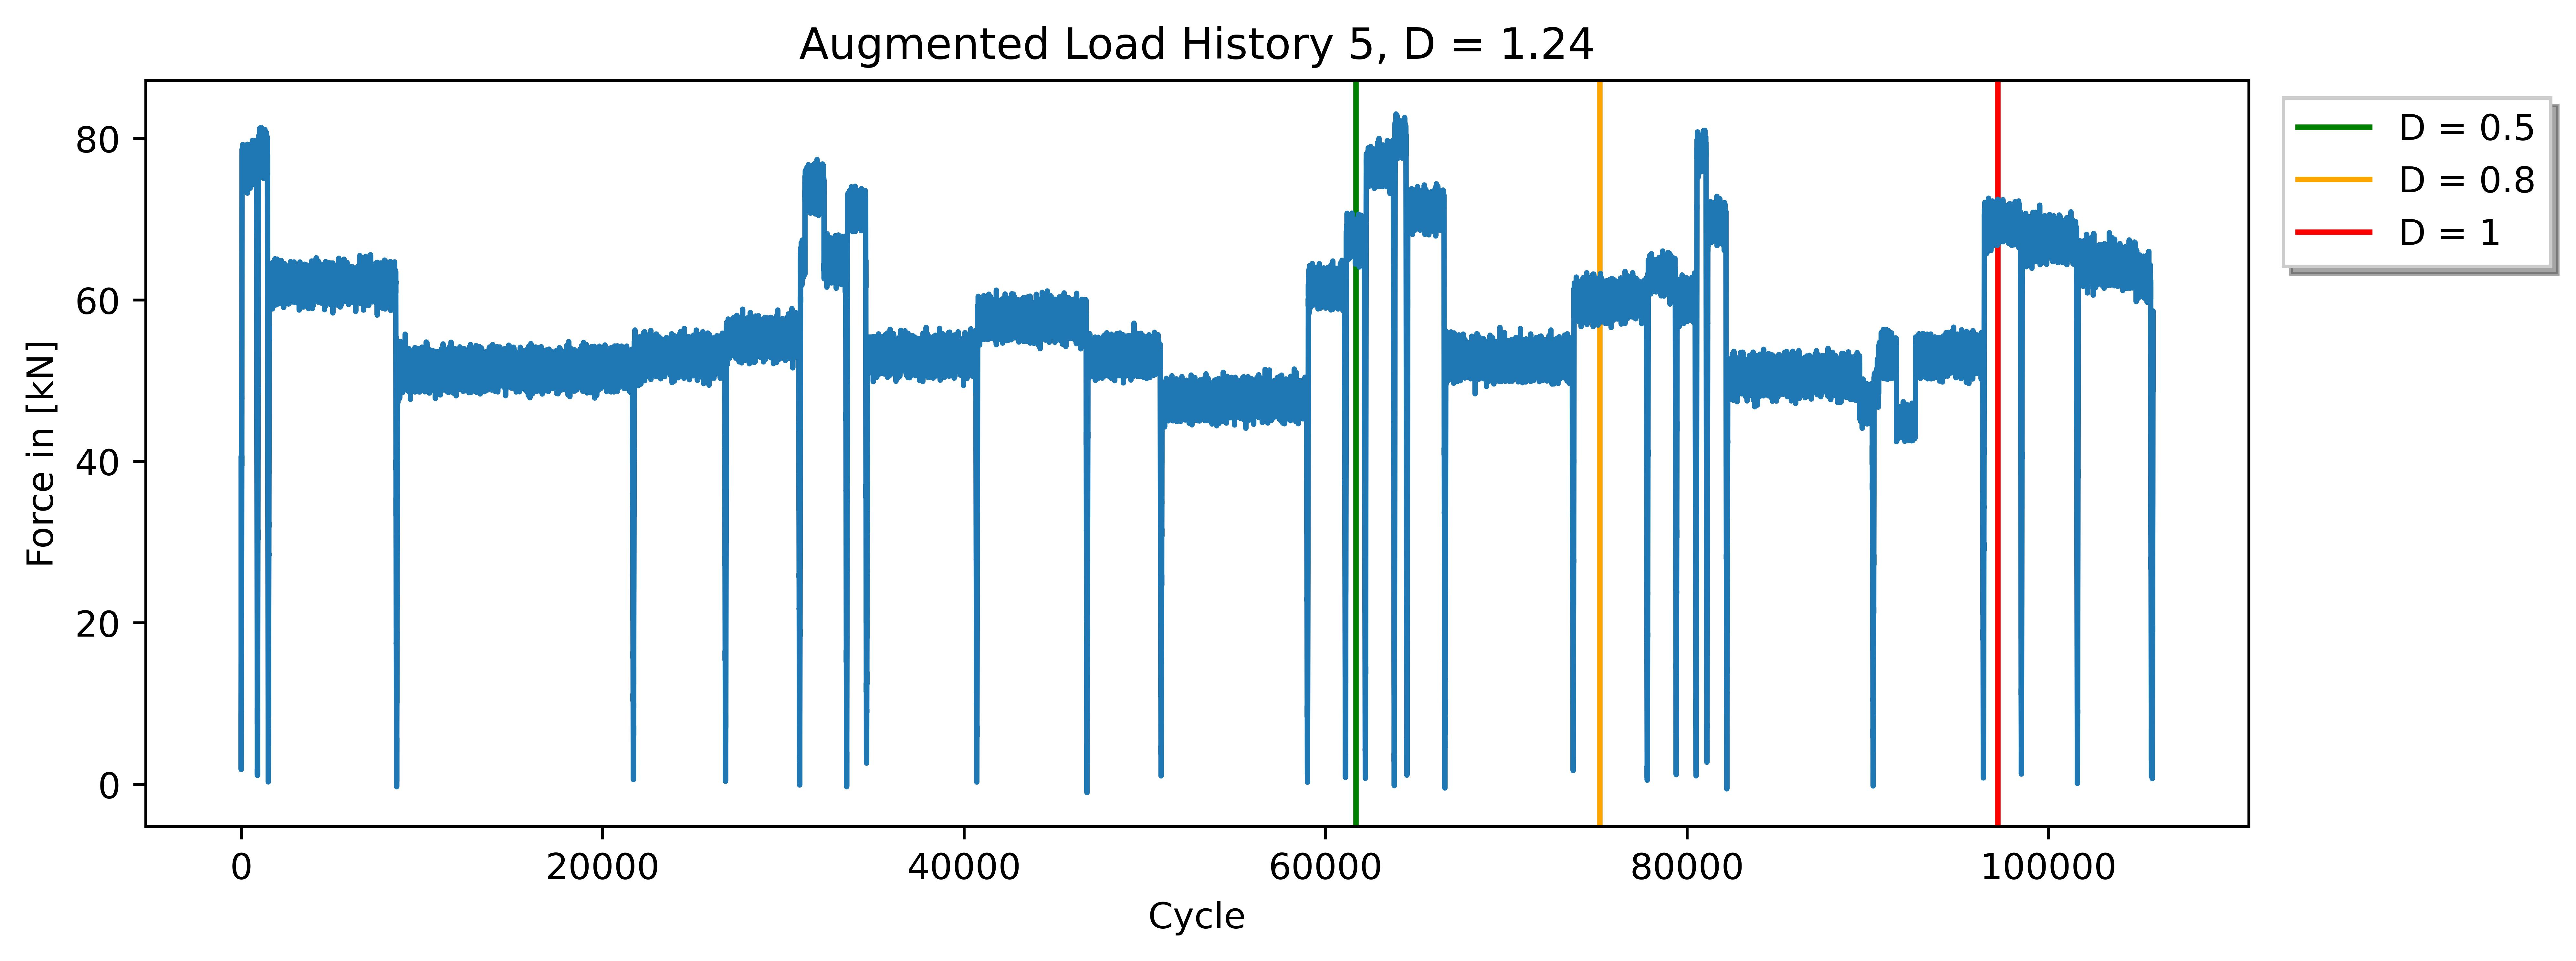
\includegraphics[width=1\linewidth]{IMGs/Verlauf_5_shift_partial.jpg}
	\caption{Load sequence with partial shift}
	\label{fig:Verlauf_5_shift_partial}
\end{figure}

The fourth step is a partial cutout, where a random section of length of 1 \% of the total length is cut out of the sequence. In this step, the damage sum D is always decreased. Figure \ref{fig:Verlauf_5_cutout} shows how the loading sequence is transformed with partial cutouts.

\begin{figure}[H]
	\centering
	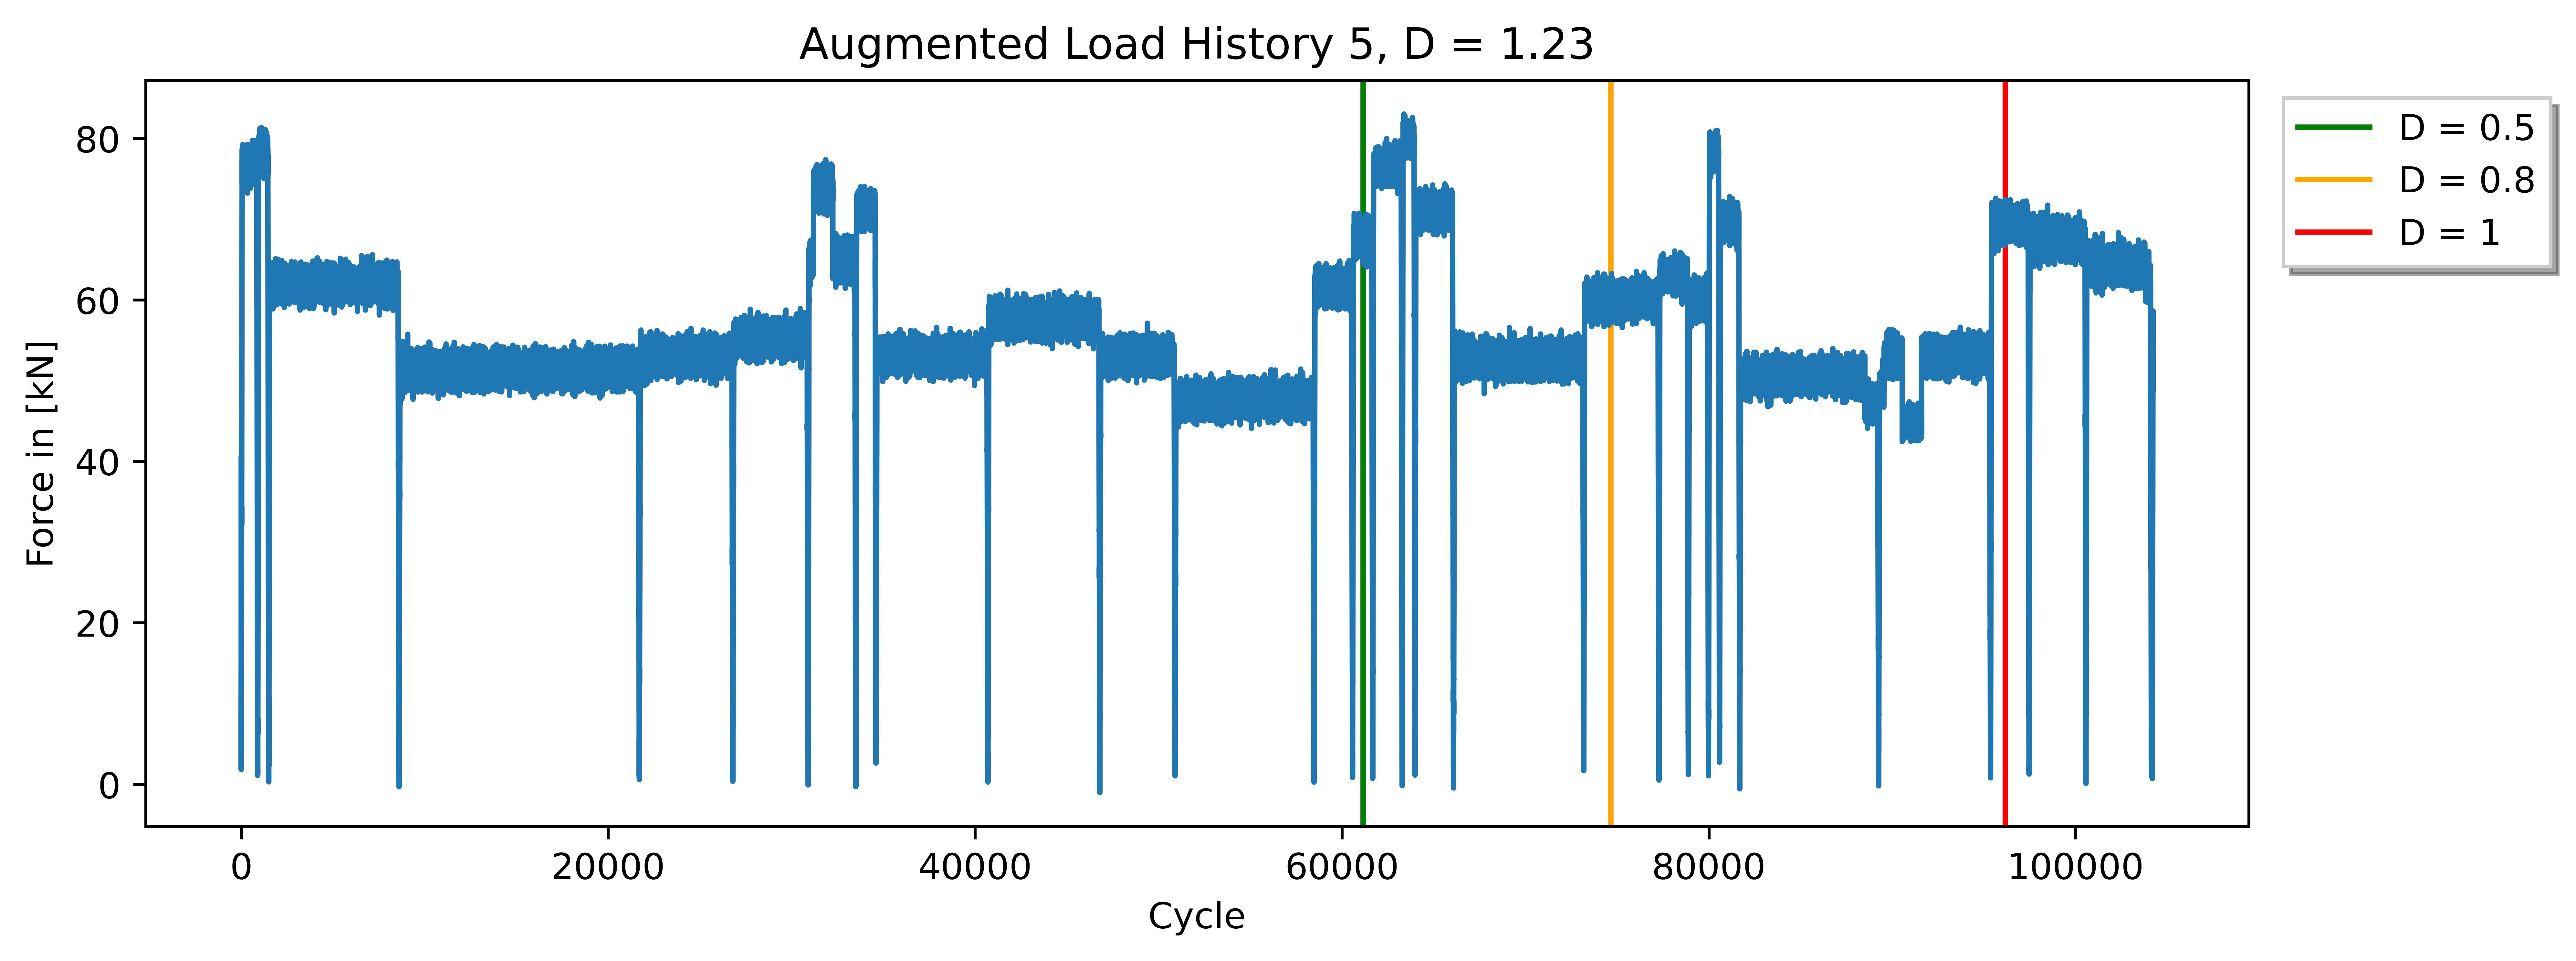
\includegraphics[width=1\linewidth]{IMGs/Verlauf_5_coutout.jpg}
	\caption{Load sequence with partial cutouts}
	\label{fig:Verlauf_5_cutout}
\end{figure}

The next step is the addition of a vector whose values are either going from positive to negative or from negative to positive over its length. It is essentially weighing the values of the load sequence over its length. By adding that vector to the load sequence, some values are increased while other are decreased. 

At first, a random variable decides if the sequence is tilted up (from negative to positive) or down (going from positive to negative). In the case of an upward shift, the start values of that vector are random variables selected from a uniform distribution in the range [-0.2, 0]. The last value is selected from a uniform distribution in the range [0, 0.2]. In the case of a downward shift, the ranges are switched.
The values between are interpolated accordingly with a constant step size.


Figure \ref{fig:Verlauf_5_tilt} shows all the previously mentioned DA-steps combined.

\begin{figure}[H]
	\centering
	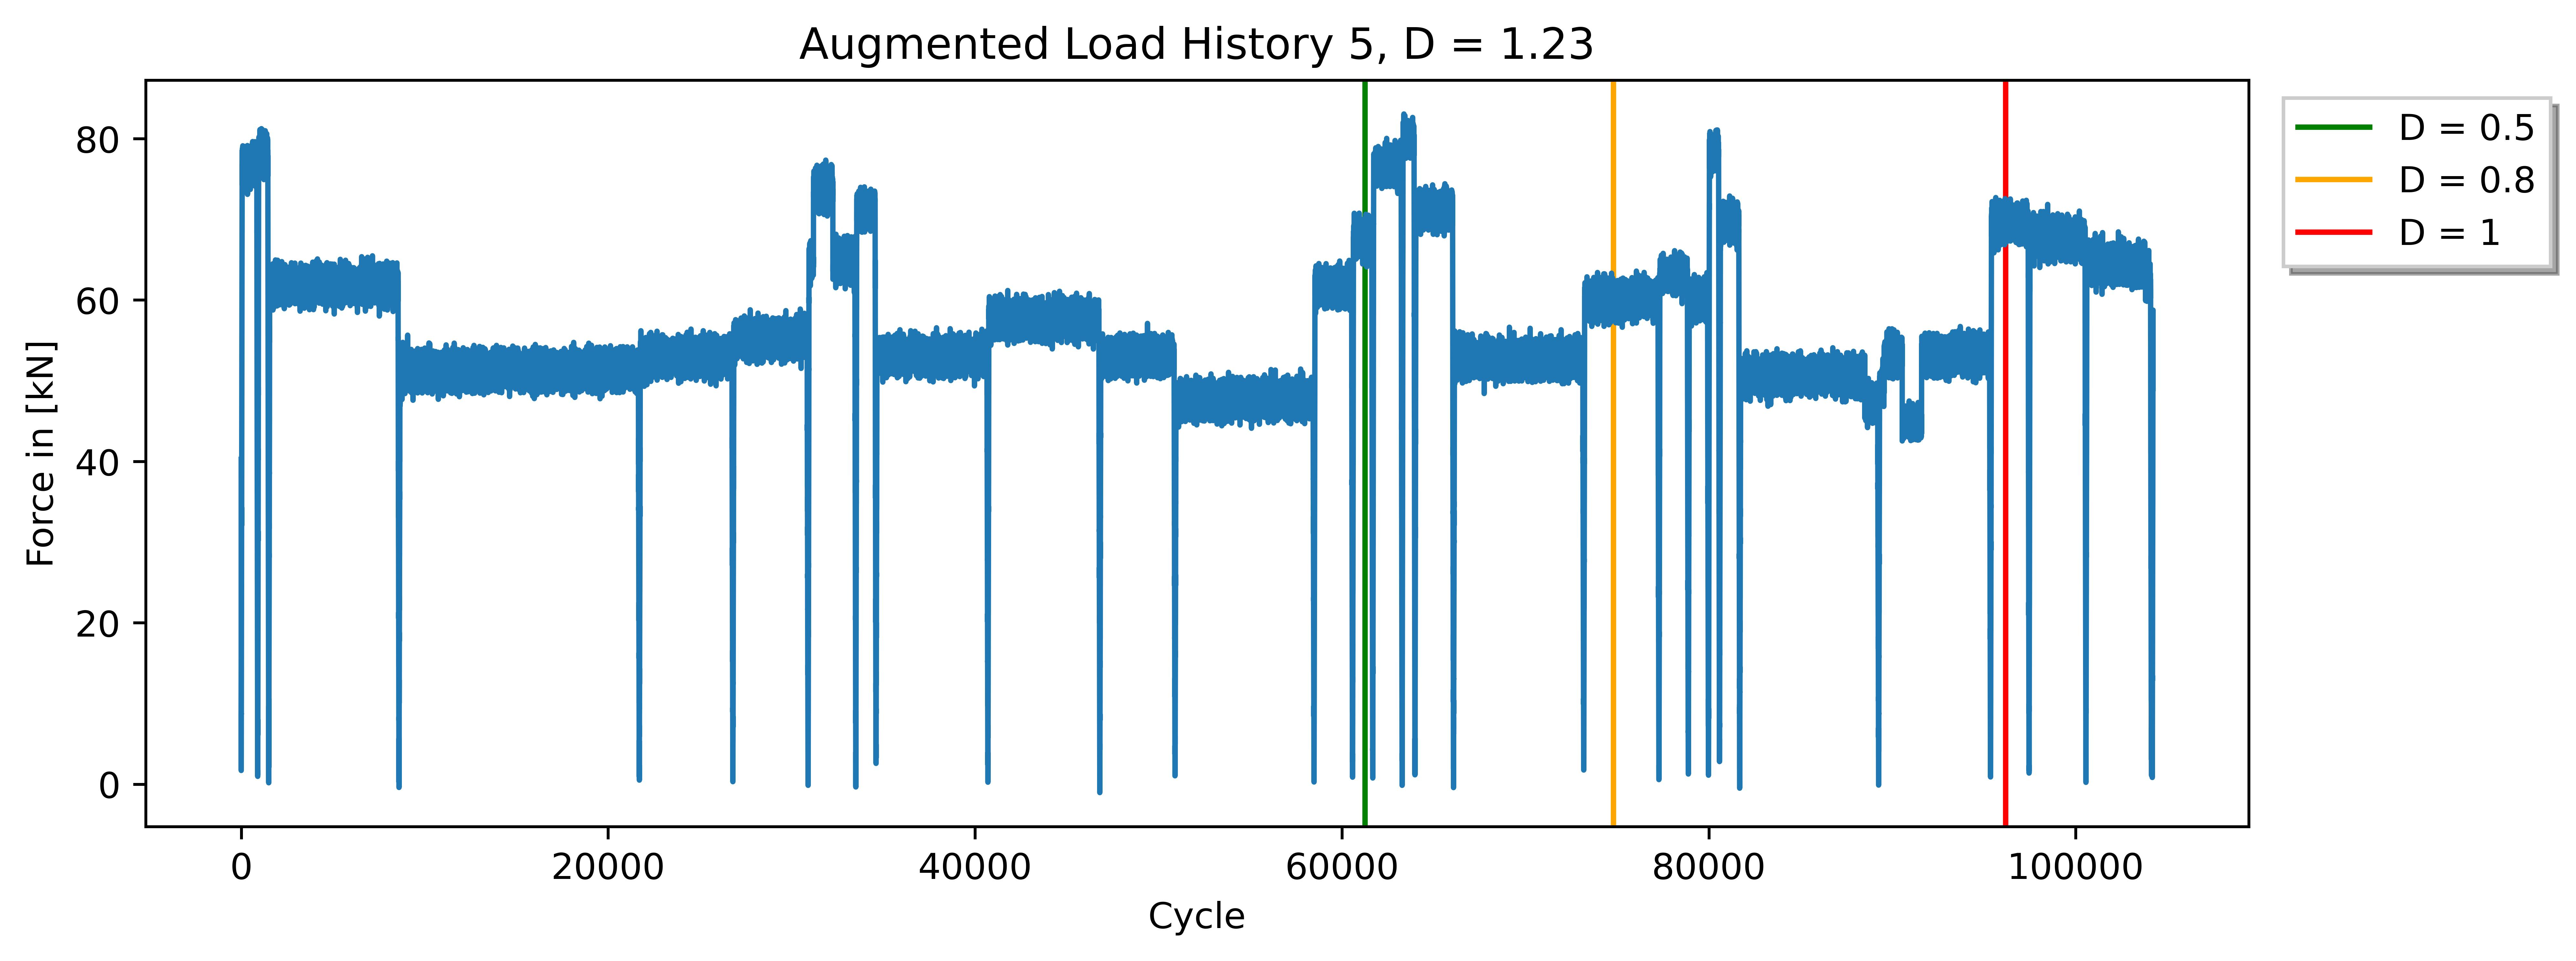
\includegraphics[width=1\linewidth]{IMGs/Verlauf_5_tilt.jpg}
	\caption{Load sequence with tilt}
	\label{fig:Verlauf_5_tilt}
\end{figure}

When comparing the original and the augmented load sequence, the visual difference is low. This is due to the fact that damage sum D must not change more that 10 \% of its original value. Only load sequences that fulfill this criteria are accepted into the training datasets.
To filter out all sequences that are off by 10 \% the original damage sum D and damage sum D after augmentation are compared.
If the ratio falls within [0.9, 1.1] the final step is applied.


The last step is dimensionality reduction, as described in chapter \ref{prep_class}. In this case, every 300\(^{th}\) point in that sequence is kept. This step is effectively reducing the length of the sequence by 300. For the last comparison of the damage sum D, the denominator in the Miner rule must be multiplied by the step size. Again only if the ration falls within [0.9, 1.1], it is accepted into the data-set. 

Figure \ref{fig:Verlauf_5_reduced} shows the load sequence in its reduced form. Notice that the characteristics of the original load sequence are still present.
 
\begin{figure}[H]
	\centering
	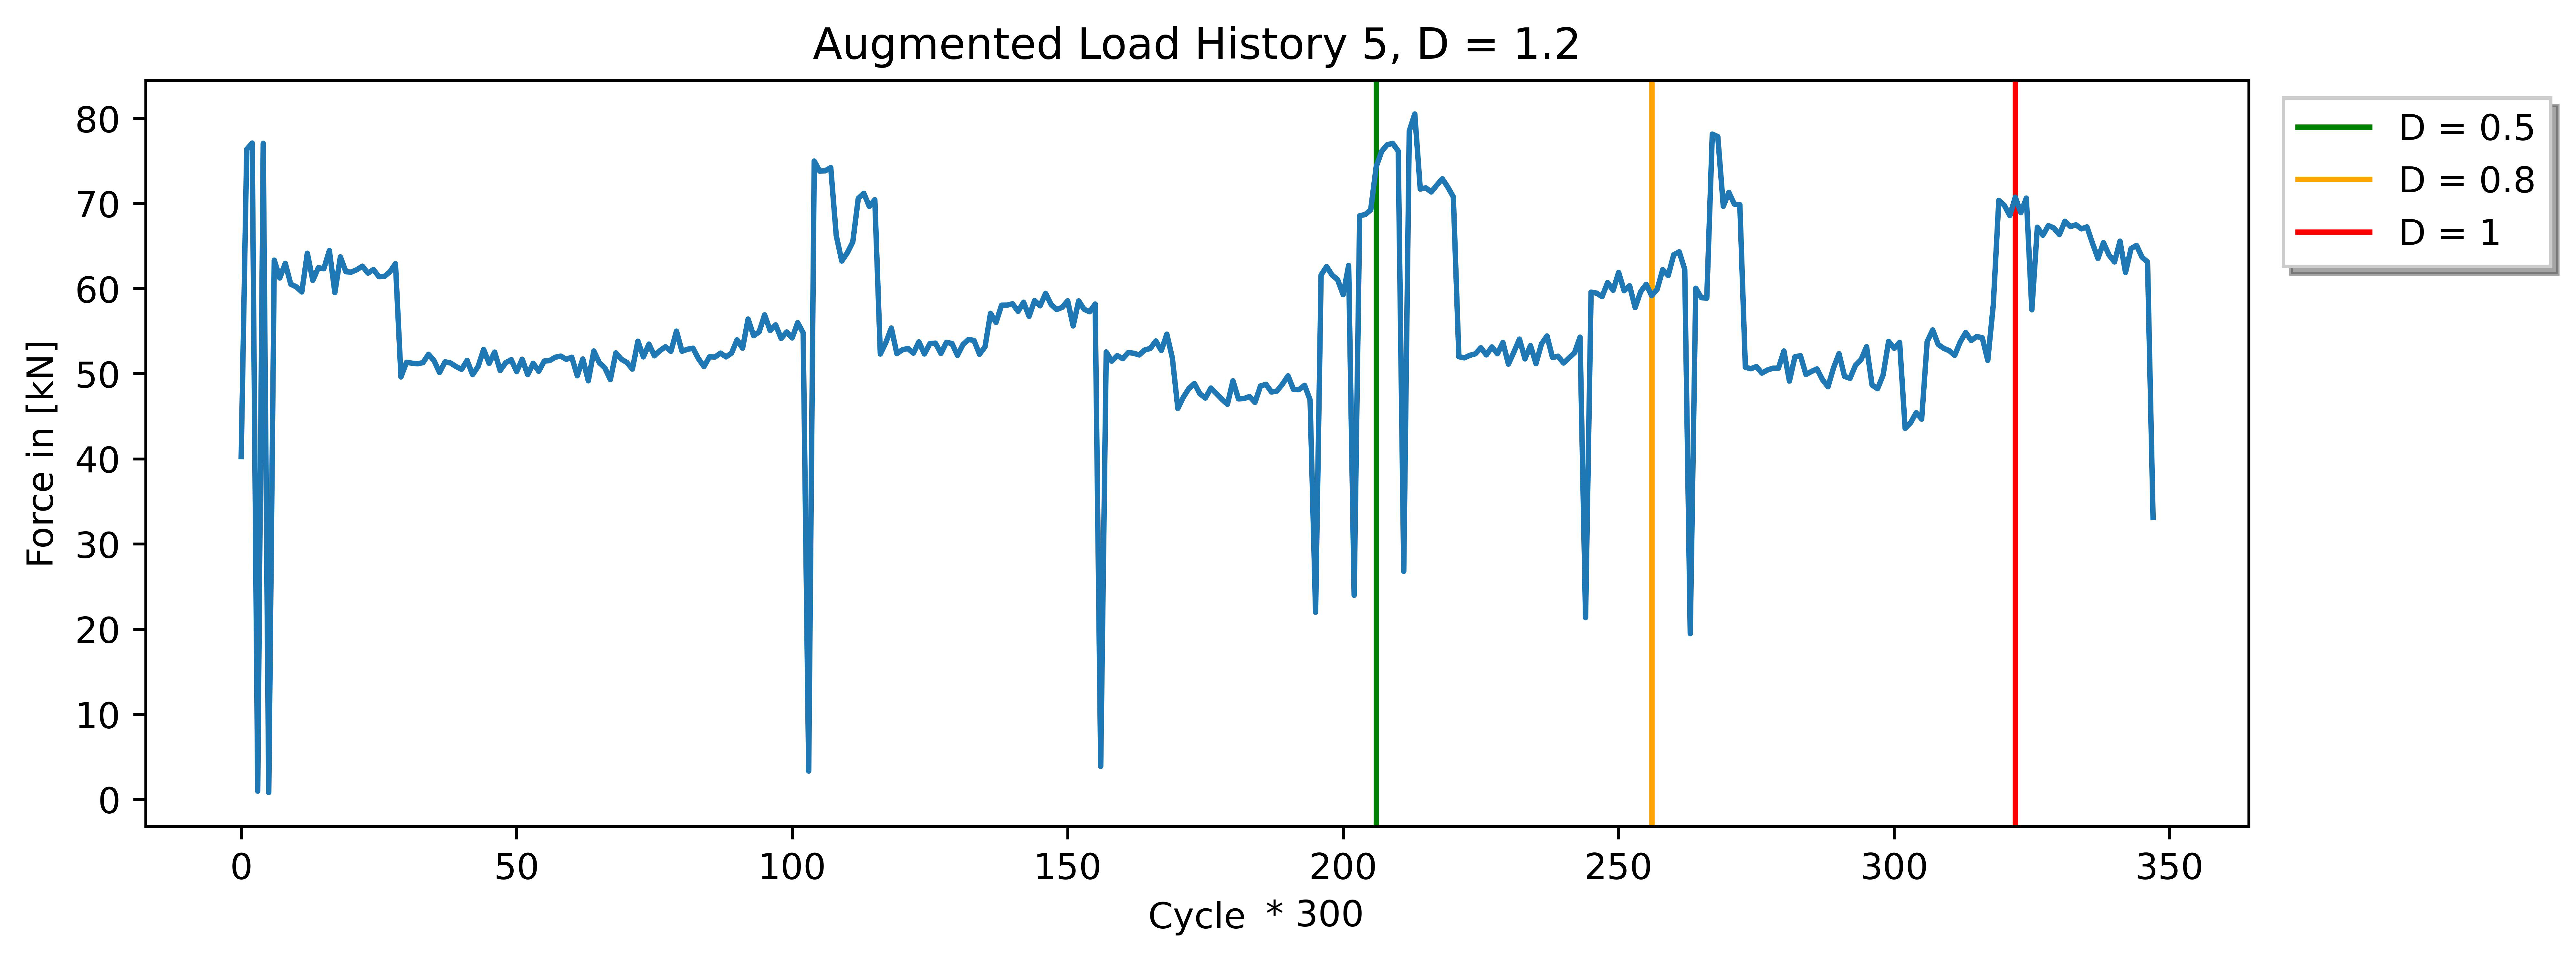
\includegraphics[width=1\linewidth]{IMGs/Verlauf_5_reduced.png}
	\caption{Load sequence after dimensionality reduction}
	\label{fig:Verlauf_5_reduced}
\end{figure}

Each load sequence is augmented with the described procedure 25 times. In the end, 25 individual instances can be present in the datasets if none of the augmented ones are filtered out. 
The accepted load sequences are saved as a np-array in a new separate folder. The name of the np-file follows the following pattern: [class\_idx.np]. "class" is the class to which the loading sequence belongs to according to table \ref{DamageClass} and "idx" is a counting index that is increasing from 0 to n to keep track of the number of data samples.

Figure \ref{fig:3in1} shows only three out of those 25 augmented sequences in one plot to highlight the differences in each sequence.
Notice how the points of damage sum D of 0.5, 0.8 and 1 vary in their positions, but the characteristics of the original load sequence are kept.

\begin{figure}[H]
	\centering
	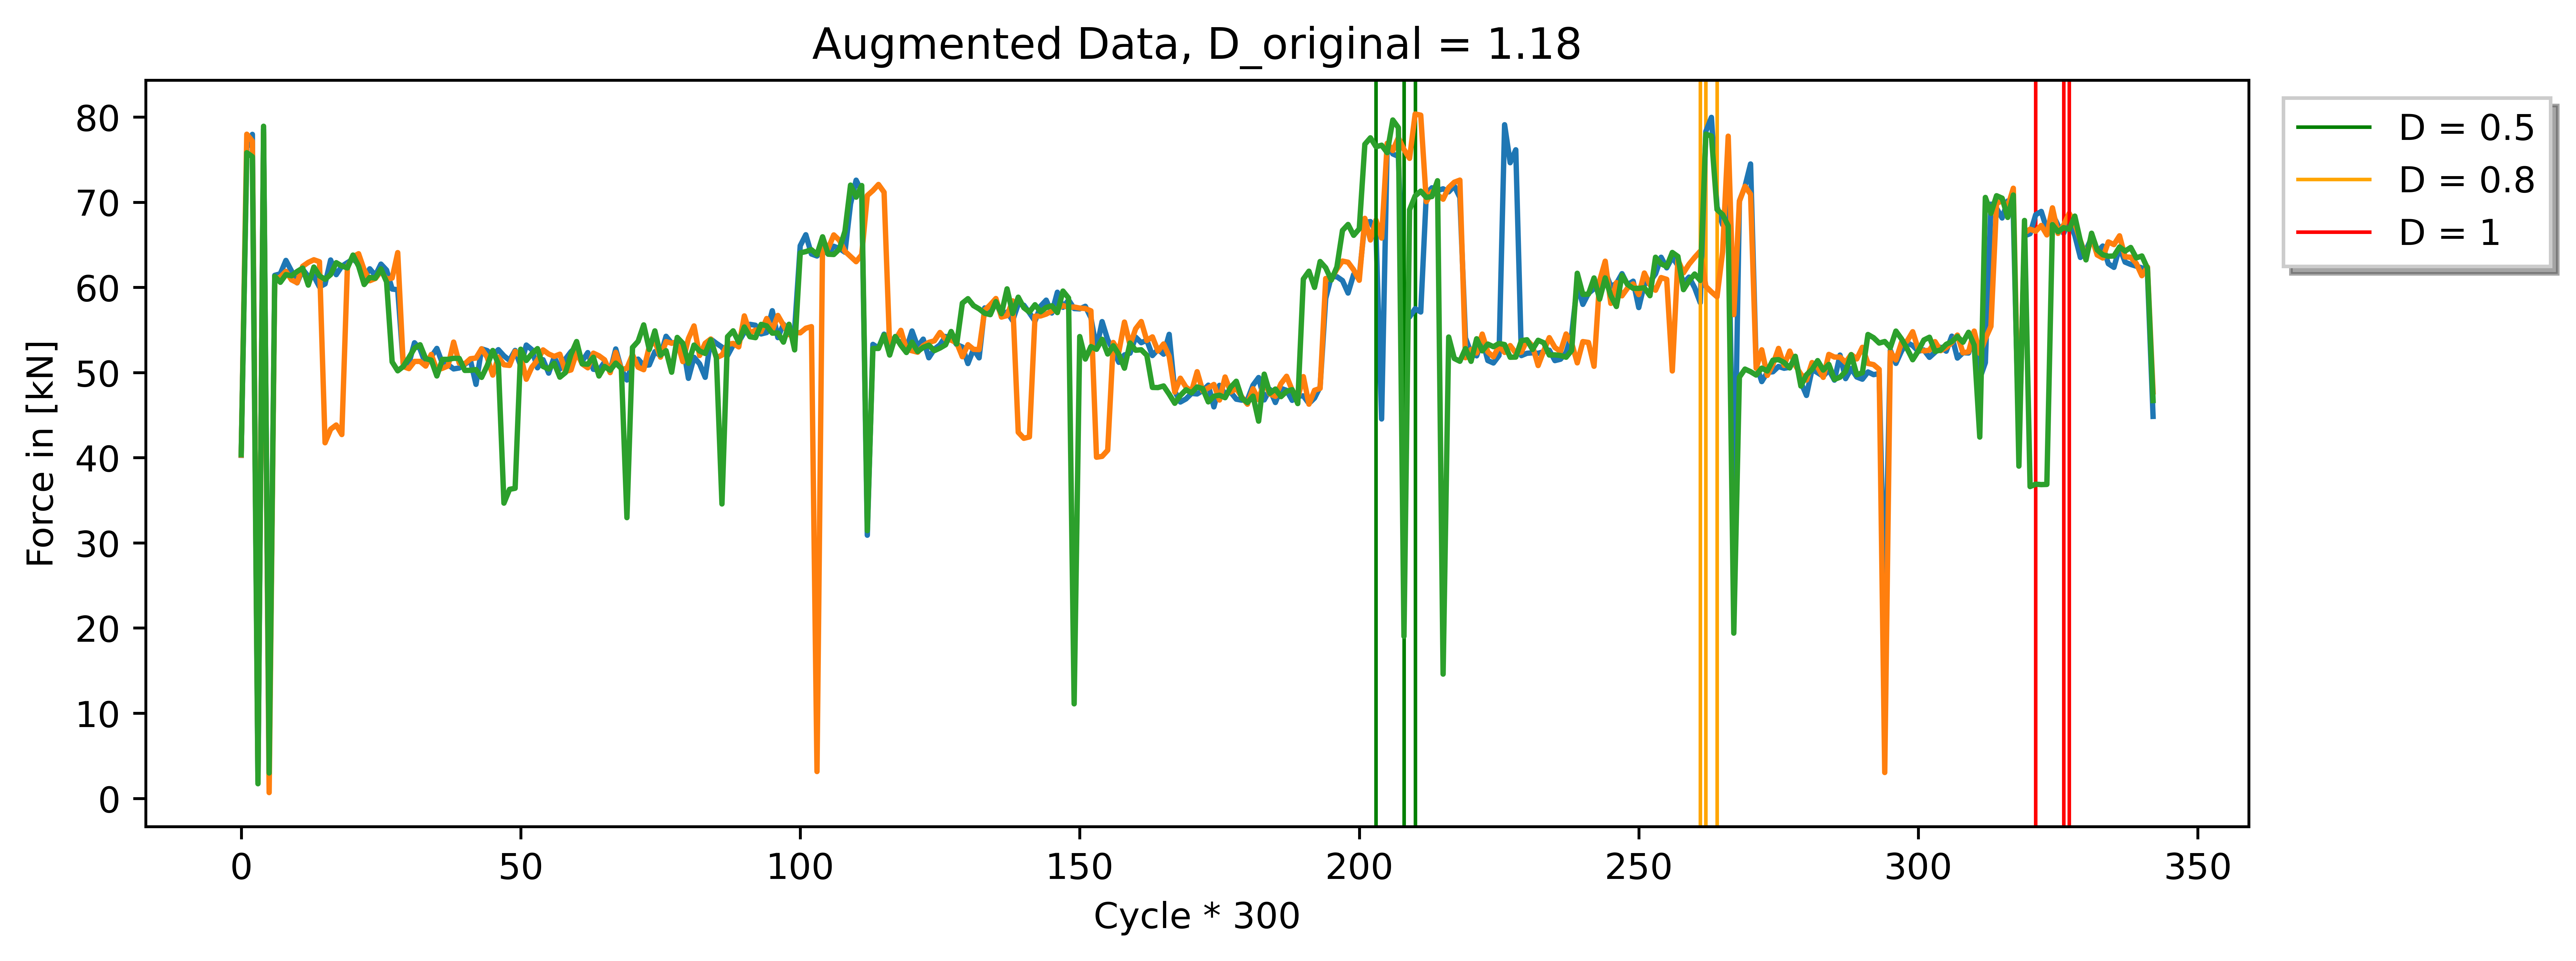
\includegraphics[width=1\linewidth]{IMGs/Augmented_5.png}
	\caption{Differences in augmented load sequences}
	\label{fig:3in1}
\end{figure}

Figure \ref{fig:allDA} shows all performed DA-steps in a schematic diagram.

\begin{figure}[H]
	\centering
	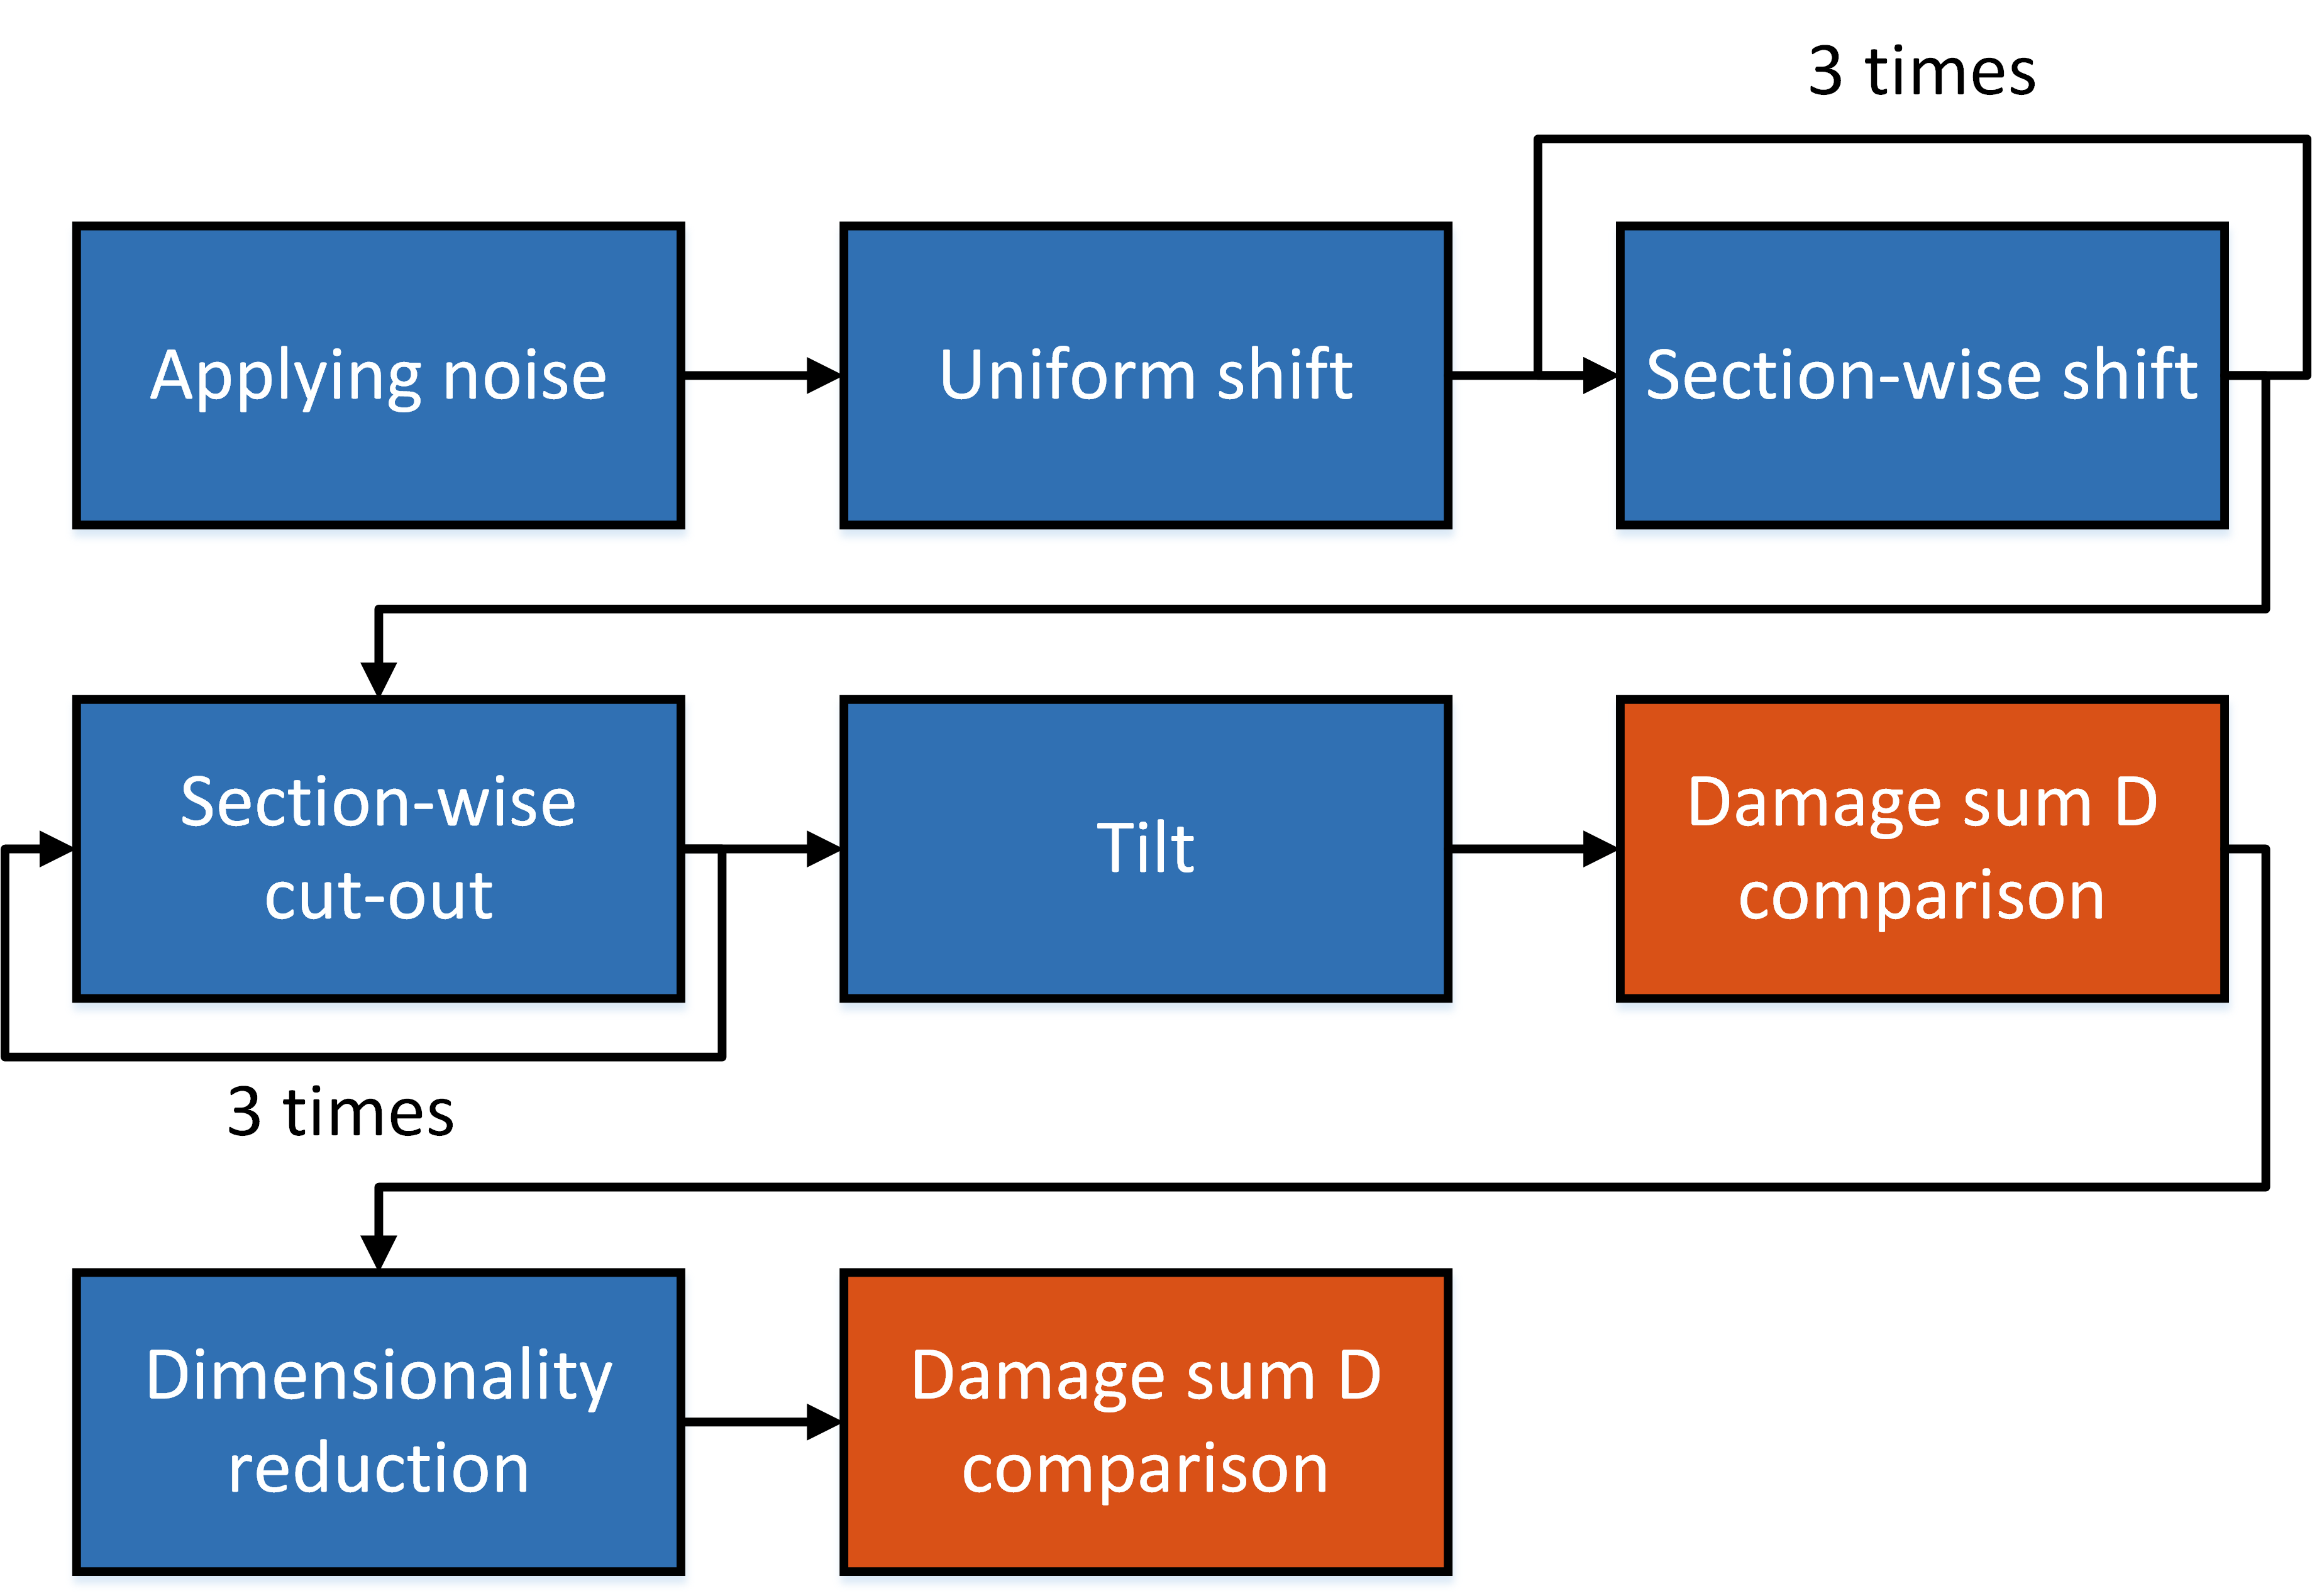
\includegraphics[width=0.7\linewidth]{IMGs/Augmentation.png}
	\caption{Augmentation procedure}
	\label{fig:allDA}
\end{figure}

From the original 14 load sequences, on average, 200 augmented sequences are created. This means that 150 out of 350 load sequences do not meet the requirement that the damage~sum~D is not significantly different from the original load sequence. 
The goal is to augment the load sequence as much as possible, while at the same time retaining the damage sum D and the characteristics of every load sequence. 


The average length on the load sequences after dimensionality reduction is 320 data points. The shortest load sequence has 66 data points and the longest one has 1000 data-points. This large difference comes from the fact that load sequence number 4 (see table \ref{DamageSUMS}) failed at a very high damage sum D while load sequence number 12 failed at a very low damage sum D.

One challenge when applying the selected DA-techniques is that a small alteration in damage sum~D in load sequences can have a very large relative change compared to the original damage~sum~D. For example, sequence number 12 has a damage sum D of 0.73 and after DA a damage sum of 0.82. The absolute change in damage sum D is 0.09. But when looking at the ratio, (0.82/0.73 = 1.12) the augmented load sequence is accepted into the training set. Thus, almost no augmented elements of sequence 12 are present in the training data set. The same problem is present, but less pronounced, with other sequences with low damage sum D.



\section{Training and Validation}
When having an unfinished load sequence that needs to be analyzed, chapters \ref{prep_class} and \ref{PrRe} explain that the classifier and regressor are trained specifically for that individual load sequence. This is because the training set is adapted to the current damage sum D of the unfinished load sequence.

For testing purposes, the damage sum D (which would have come from the unfinished load sequence) is manually set to 0.6
The success of the classifier and regressor is analyzed by splitting the data into a test-set and training-set. 
20~\% of the data is given to the test-set and 80~\% to the training-set.

The training-set contains on average: 50 elements of class -1, 30 elements of class 0 and 90 elements of class 0. This ratio comes directly from the distribution of the original data-set where most load sequences failed at a damage sum D higher than 1.1.

\subsection{Training of the Classifier}
To train the classifier, the augmented load sequences are loaded into one list of arrays. The label of the array is extracted from the names of the files created in the augmentation step and also stored in an array. 

The load sequences are in their full length and need to be shortened to the length where the damage sum D is equal to 0.6 to be comparable to the unfinished load sequence. Note that in this case, the unfinished load sequence corresponds to the sequences in the test-set. 


The dataset is divided into a training- and test-set with the help of a prebuilt train-test-split function taken from \cite{SKlearn}. Table \ref{methods} shows the ten classifiers that are implemented to compare their individual performance:

%\begin{itemize} 
%	\itemsep-0.5em 
%	\item KNeighborsTimeSeriesClassifier \cite{tslearn}
%	\item TimeSeriesSVC \cite{tslearn}
%	\item AdaBoostClassifier \cite{SKlearn}
%	\item GradientBoostingClassifier \cite{SKlearn}
%	\item RandomForestClassifier \cite{SKlearn}
%	\item XGBoost\cite{XG}
%	\item Neural Net \cite{SKlearn}
%	\item GaussianNB \cite{SKlearn}
%	\item QuadraticDiscriminantAnalysis \cite{SKlearn}
%	\item KNeighborsClassifier \cite{SKlearn}
%\end{itemize}


\begin{table}
	\begin{center}
		\begin{tabular}{|| l | l ||}\hline
			\rule{0pt}{2ex}KNeighborsTimeSeriesClassifier \cite{tslearn} & TimeSeriesSVC \cite{tslearn}\\	\hline
			AdaBoostClassifier \cite{SKlearn} & GradientBoostingClassifier \cite{SKlearn} \\ \hline
			RandomForestClassifier \cite{SKlearn} & XGBoost\cite{XG}\\ \hline
			Neural Net \cite{SKlearn} & GaussianNB \cite{SKlearn} \\ \hline
			QuadraticDiscriminantAnalysis \cite{SKlearn} & KNeighborsClassifier \cite{SKlearn} \\ \hline
		\end{tabular}
		\caption{Implemented Methods for Classification}
		\label{methods}
	\end{center}
	\vspace{-4mm}
\end{table}

Only the "KNeighborsTimeSeriesClassifier" and "TimeSeriesSVC" are capable of accepting input vectors that have a varying length. To use the remaining classifiers, the load sequences are brought to the same length by pre-pending zeros, so that the overall length is equal to the longest sequence. Note that the length is defined by the longest load sequence in both of the datasets (train- and test-set).




\subsection{Training of the Regressor}
The training set of the regressor is dependent on the result of the classifier. For analysis purposes, the performance is analyzed by predicting the SOH on all three possible classes. 

For a predicted class, for example class 1, only the load sequences are loaded that belong to that class. In each load sequence, a random point is selected, and the label is calculated by the label function as described in chapter \ref{PrRe}. The array is shortened to the randomly selected point and stored in a list. The corresponding label is stored in an array. From each load sequence, four such frames are selected.

The analyzed regressors for predicting the SOH are:
\begin{itemize} 
	\itemsep-0.5em 
	\item AdaBoostRegressor \cite{tslearn}
	\item RandomForestRegressor \cite{tslearn}
\end{itemize}

The library "TSlearn" \cite{tslearn} contains a regressor called "TimeSeriesSVR", which is capable of working with input vectors of different lengths. The issue is that the maximum length must not exceed 450 elements. Because some arrays exceed this length, only two selected regressors from SKlearn \cite{SKlearn} are tested. To bring all arrays to the same length, a zero-padding method is employed, just as in the classification approach.

\section{Analysis and Discussion of the Results}
\subsection{Results of Classification}
To get an accurate evaluation of the performance of the selected classifiers, each model is trained and tested 25 times on a different data-set. This means that the data augmentation step of all load sequences is performed every time before the training of a classifier starts.
By doing that, the train- and test-set are varied. Another way to get the average performance is k-fold cross-validation as described in chapter \ref{KCV}. Due to the ability to generate variations in data, the k-fold cross-validation approach is disregarded. By averaging the performance over 25 iterations on the test-set, an accurate average performance is calculated. 

The average individual performance of all tested classifiers is shown in figure \ref{fig:avgperf}. 
A score of 1 means a correct classification of all sequences. Value in the pot is a ratio of correctly predicted classes to all predictions.

\begin{figure}[H]
	\centering
	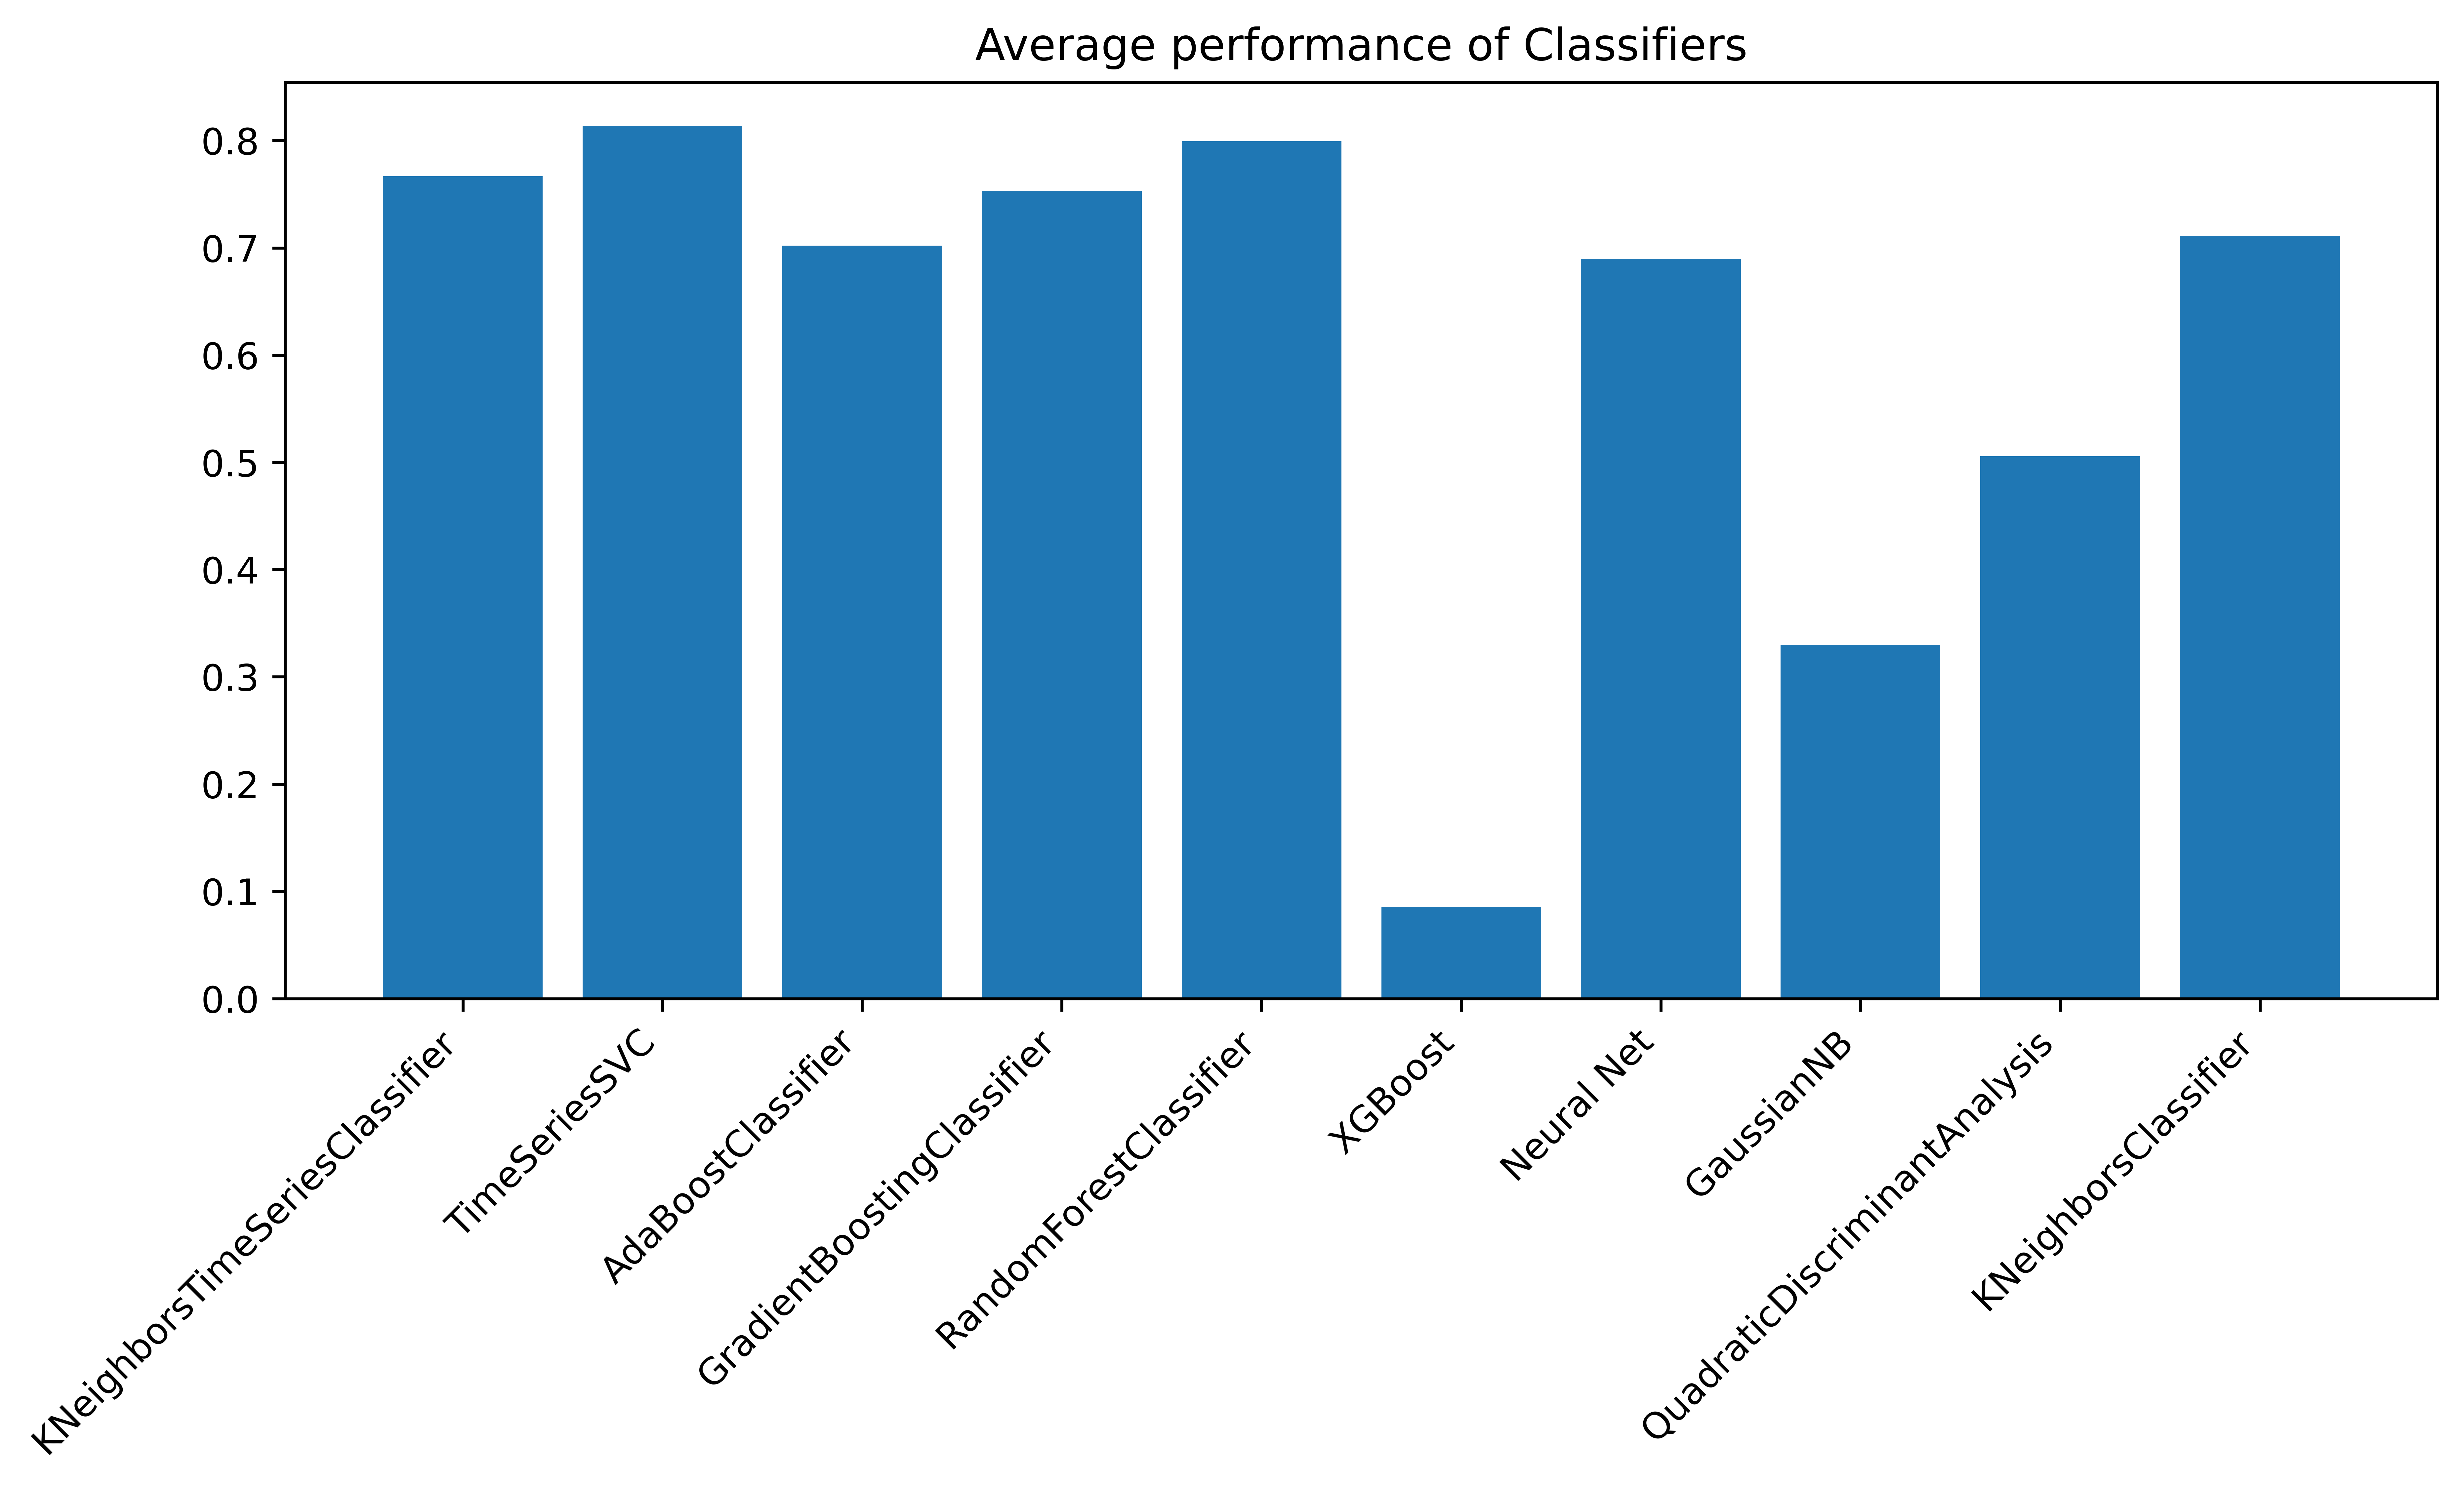
\includegraphics[width=1\linewidth]{IMGs/Average_performance_CLASS.png}
	\caption{Average performance of predicting the correct class for each classifier}
	\label{fig:avgperf}
\end{figure}

When looking at the results, most of the classifiers are capable of predicting the correct class for the load sequences in the test-set of up to 80 \% of the time. 
It is noticeable that the two first classifiers that are working with input vectors of varying length are as capable as the classifiers that require constant dimensions. The best performance is achieved by "TimeSeriesSVC" from \cite{tslearn} which predicted the correct class 81.3 \% of the time. The worst performance was achieved by "XGboost" with only 8.5 \%. This is a noticeable result because an average score of 33 \% is expected when the labels are predicted at random. 

Table \ref{score} shows the analyzed classifiers sorted by performance. 

\begin{table}
	\begin{center}
		\begin{tabular}{|| l | l ||}
			\hline
			\rule{0pt}{2ex}Classifier & Average performance\\
			\hline
			\hline
			\rule{0pt}{2ex}TimeSeriesSVC & 81.3 \%\\	\hline
			RandomForestClassifier & 79.9 \% \\ \hline
			KNeighborsTimeSeriesClassifier & 76.6 \%\\ \hline
			GradientBoostingClassifier & 75.3 \%\\ \hline
			KNeighborsClassifier & 71.1 \%\\ \hline
			AdaBoostClassifier & 70.1 \% \\ \hline
			Neural Net & 68.9 \% \\ \hline
			QuadraticDiscriminantAnalysis & 50.5 \% \\ \hline
			GaussianNB & 32.9 \% \\ \hline
			XGBoost & 8.5 \% \\ \hline
			\hline
		\end{tabular}
		\caption{Average performance of classifiers}
		\label{score}
	\end{center}
	\vspace{-4mm}
\end{table}
\newpage
\subsection{Results of Regression}

The regressors are trained for each possible class and evaluated on their performance. The performance is averaged over 25 trainings to get an accurate average score for the regressors. The score is obtained by averaging the mean-square error of the prediction for each class.

Figure \ref{fig:avgperf_reg} shows the result of the averaged training. The predictions of the correct SOH in classes -1 and 1 are more accurate than in class 0. One possible explanation for this performance is the previously mentioned disparity in elements in each class. Class 1 and class~-1 have more data points and thus allow for a better prediction. Both regressors show similar performance in each class.

\begin{figure}[H]
	\centering
	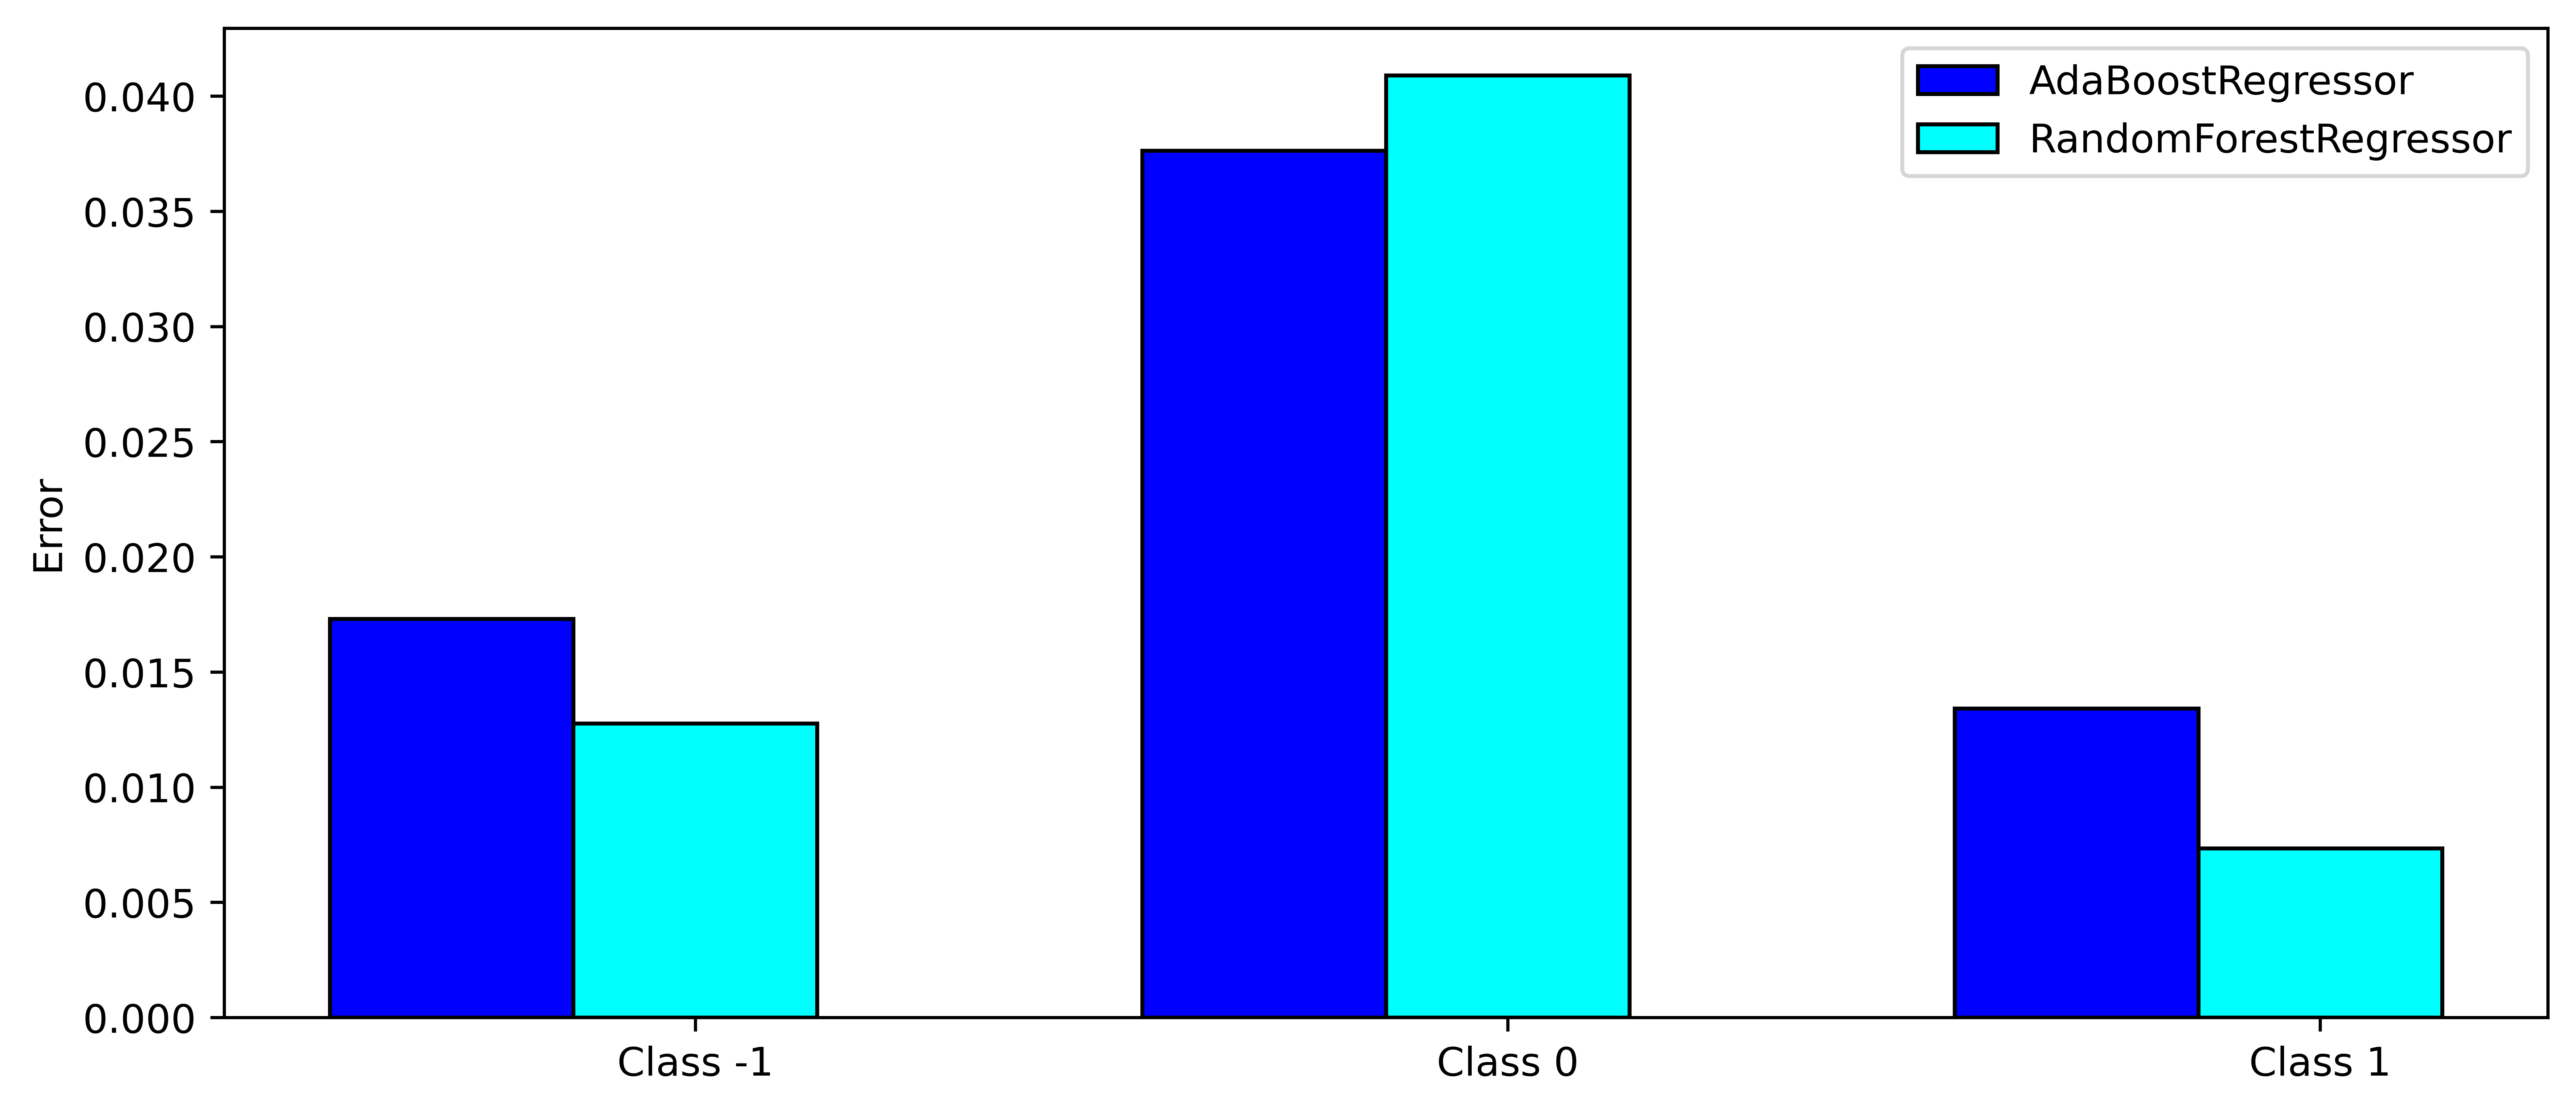
\includegraphics[width=1\linewidth]{IMGs/Average_performance_REG.png}
	\caption{Average performance of each regressor for predicting the SOH in each class}
	\label{fig:avgperf_reg}
\end{figure}
\subsection{Critical Discussion of Results}

The tested methods prove to return accurate results in classification and regression. One possible reason for that is that the implemented DA steps do not alter the structure of the loading sequence enough to be seen as a completely different load sequence. Thus, if an augmented element of a load sequence is in the training-set and testing-set, the ML models do not need to have the ability to generalize to predict the correct class for that sequence. 

When predicting the SOH the inputs from test- and training-set have significant differences in length. Thus the same problem of over-fitting is not present. For a more accurate result and better performance of the ML models more data is necessary. As mentioned before only 14~load sequences were available which makes the training of the ML models to generalize well, a difficult task.   

